\documentclass{article}

%% Language and font encodings
\usepackage[english,spanish]{babel}
\usepackage[utf8]{inputenc}
\usepackage[T1]{fontenc}
\usepackage{enumitem}

%% Sets page size and margins - Reduced margins for more compact layout
\usepackage[a4paper,top=2cm,bottom=1.5cm,left=2cm,right=2cm,marginparwidth=1.5cm]{geometry}

%% Useful packages
\usepackage{amsmath}
\usepackage{graphicx}
\usepackage[colorlinks=true, allcolors=blue]{hyperref}
\usepackage{longtable}
\usepackage{array}
\usepackage{booktabs}
\usepackage{float}
\usepackage{subcaption}
\usepackage{pgfplots}
\usepackage{tikz}
\pgfplotsset{compat=1.17}

% Compact spacing
\setlength{\parskip}{0.3em}
\setlength{\itemsep}{0.1em}
\usepackage{titlesec}
\titlespacing*{\section}{0pt}{1em}{0.5em}
\titlespacing*{\subsection}{0pt}{0.8em}{0.3em}

\title{Caso de Estudio: Pruebas de Regresión Visual en Interfaces Gráficas\\
\large Comparación de Herramientas Percy Cloud, Playwright y BackstopJS}

\author{Mesias Mariscal, Denise Rea, Julio Viche}

\date{\today}

\begin{document}
\maketitle

\section{Introducción}

Las pruebas de regresión visual son una técnica fundamental para detectar cambios no deseados en las interfaces gráficas de aplicaciones web. A diferencia del testing funcional tradicional, estas pruebas se enfocan en verificar que la apariencia visual de los componentes se mantenga consistente después de modificaciones en el código.

Este caso de estudio presenta una comparación empírica de tres herramientas líderes en el mercado: Percy Cloud, Playwright Visual Testing y BackstopJS. La evaluación se realizó utilizando el proyecto FAESign, un sistema de firma electrónica desarrollado en React, aplicando metodologías científicas para garantizar resultados objetivos y reproducibles.

\subsection{Problema de Investigación}
\textbf{Pregunta guía:} ¿Es posible detectar eficazmente errores en interfaces gráficas mediante comparación visual automatizada, y cuál herramienta ofrece el mejor balance entre precisión, facilidad de uso y eficiencia técnica?

\subsection{Objetivos}
\begin{itemize}[nosep]
\item Evaluar la eficacia de tres herramientas de regresión visual en condiciones idénticas
\item Medir métricas cuantitativas de rendimiento, precisión y facilidad de implementación
\item Analizar la tasa de falsos positivos y negativos en cada herramienta
\item Implementar automatización completa con la herramienta seleccionada
\item Proporcionar recomendaciones basadas en evidencia para diferentes escenarios de uso
\end{itemize}

\section{Marco Teórico}

\subsection{Pruebas de Regresión Visual}
Las pruebas de regresión visual comparan capturas de pantalla de referencia (baseline) con capturas actuales para detectar diferencias pixel por pixel. Esta técnica es especialmente valiosa en aplicaciones web modernas donde pequeños cambios en CSS pueden tener efectos visuales no deseados.

\subsection{Tipos de Herramientas Evaluadas}
\begin{itemize}[nosep]
\item \textbf{Percy Cloud:} Servicio SaaS especializado en comparación visual con dashboard colaborativo
\item \textbf{Playwright:} Framework de testing E2E con capacidades de comparación visual integradas
\item \textbf{BackstopJS:} Herramienta open-source para regresión visual con reportes HTML detallados
\item \textbf{Loki (descartado):} Inicialmente considerado pero incompatible con React 19
\end{itemize}

\subsection{Por qué se Descartó Loki}
Durante la implementación inicial, se intentó incluir Loki como tercera herramienta de comparación. Sin embargo, se identificaron problemas críticos de compatibilidad:

\begin{itemize}[nosep]
\item \textbf{Incompatibilidad con React 19:} Loki requiere React 17 como máximo
\item \textbf{Dependencias obsoletas:} Múltiples conflictos con las dependencias del proyecto actual
\item \textbf{Falta de mantenimiento:} El proyecto no ha sido actualizado para soportar ecosistemas modernos
\item \textbf{Errores de instalación:} Fallos persistentes durante npm install debido a incompatibilidades de versiones
\end{itemize}

Por estas razones técnicas, se optó por BackstopJS como alternativa moderna y bien mantenida que ofrece funcionalidad similar con mejor compatibilidad.

\section{Metodología}

\subsection{Proyecto de Prueba: FAESign}
Se utilizó FAESign, una aplicación React para firma electrónica, como caso de estudio. El proyecto incluye:
\begin{itemize}[nosep]
\item Componentes React con estados visuales variados
\item Diseño responsivo con breakpoints móvil, tablet y desktop
\item Integración con Storybook para testing aislado de componentes
\item Pipeline CI/CD con GitHub Actions
\end{itemize}

\subsection{Configuración Experimental}
Para garantizar una comparación justa, todas las herramientas utilizaron configuraciones idénticas:

\textbf{Viewports Estandardizados:}
\begin{itemize}[nosep]
\item Móvil: 375×667px (iPhone estándar)
\item Tablet: 768×1024px (iPad estándar)  
\item Desktop: 1280×720px (Pantalla estándar)
\end{itemize}

\textbf{Navegadores de Prueba:}
\begin{itemize}[nosep]
\item Chromium (motor de Chrome/Edge)
\item Firefox (motor Gecko)
\item WebKit (motor de Safari)
\end{itemize}

\textbf{CSS de Estabilización (aplicado a todas las herramientas):}
\begin{verbatim}
*, *::before, *::after {
  animation-duration: 0s !important;
  transition-duration: 0s !important;
}
.timestamp, .date, .current-time {
  visibility: hidden !important;
}
\end{verbatim}

\subsection{Componente de Prueba: StatusMessage}
Se seleccionó el componente \texttt{StatusMessage} por sus características ideales para testing visual:
\begin{itemize}[nosep]
\item \textbf{4 variantes visuales:} success (verde), error (rojo), warning (amarillo), info (azul)
\item \textbf{Comportamiento responsivo:} Diferentes layouts según viewport
\item \textbf{Estados definidos:} Sin elementos dinámicos complejos
\item \textbf{Aislamiento:} Componente independiente sin dependencias externas
\end{itemize}

\section{Resultados Experimentales}

\subsection{Percy Cloud}

\subsubsection{Configuración e Implementación}
Percy Cloud se configuró utilizando el archivo \texttt{.percy.yml} con integración directa a Playwright:

\begin{figure}[H]
\centering
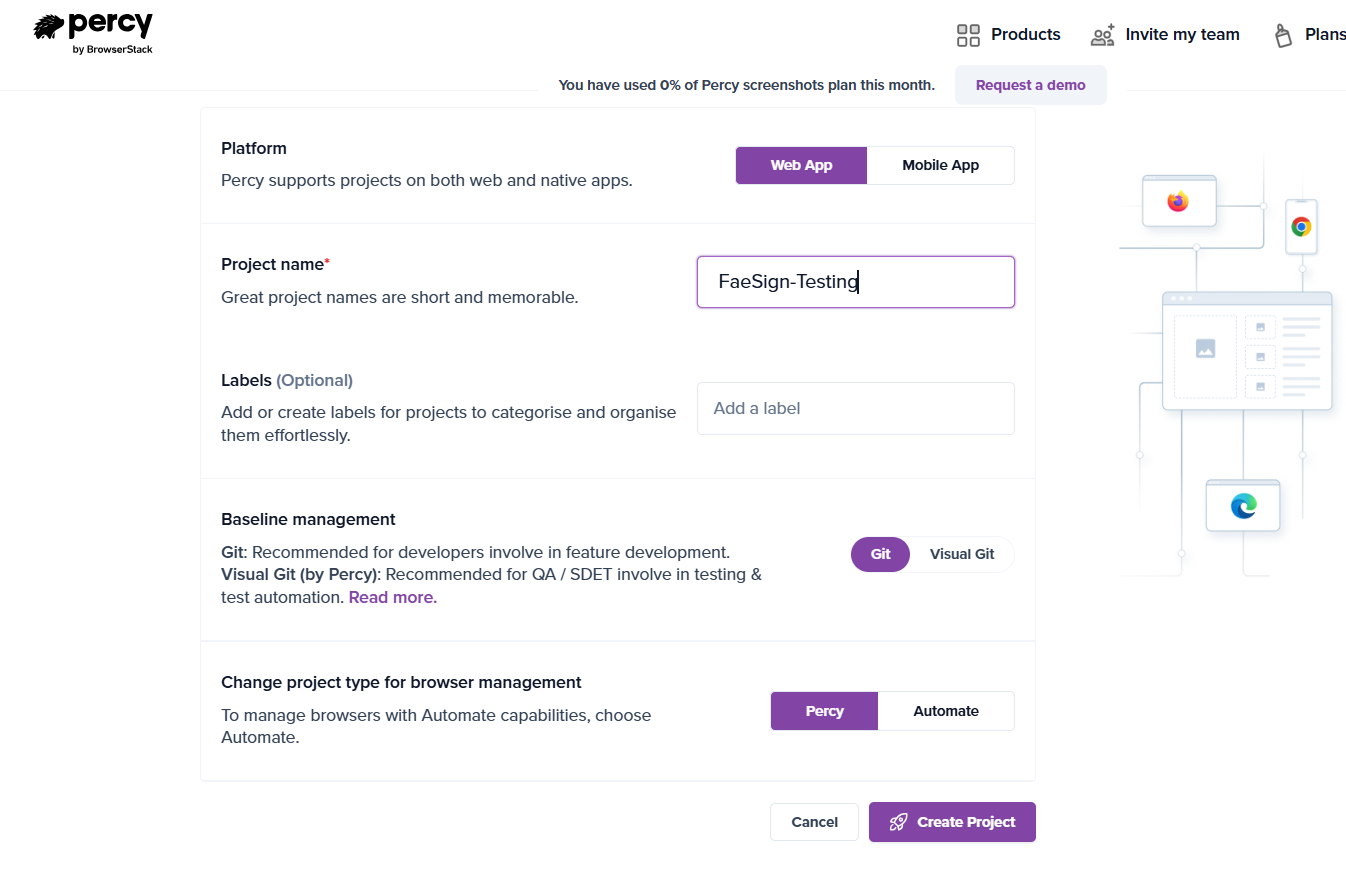
\includegraphics[width=0.8\textwidth]{percy/createProject.png}
\caption{Configuración inicial del proyecto en Percy Cloud}
\label{fig:percy-setup}
\end{figure}

\subsubsection{Resultados Cuantitativos}
\begin{itemize}[nosep]
\item \textbf{Pruebas ejecutadas:} 111 total
\item \textbf{Snapshots exitosos:} 81 (69.2\% tasa de éxito)
\item \textbf{Navegadores probados:} Chrome, Firefox, Safari
\item \textbf{Tiempo de ejecución:} 26.1 segundos
\item \textbf{Falsos positivos:} 0 detectados
\end{itemize}

\begin{figure}[H]
\centering
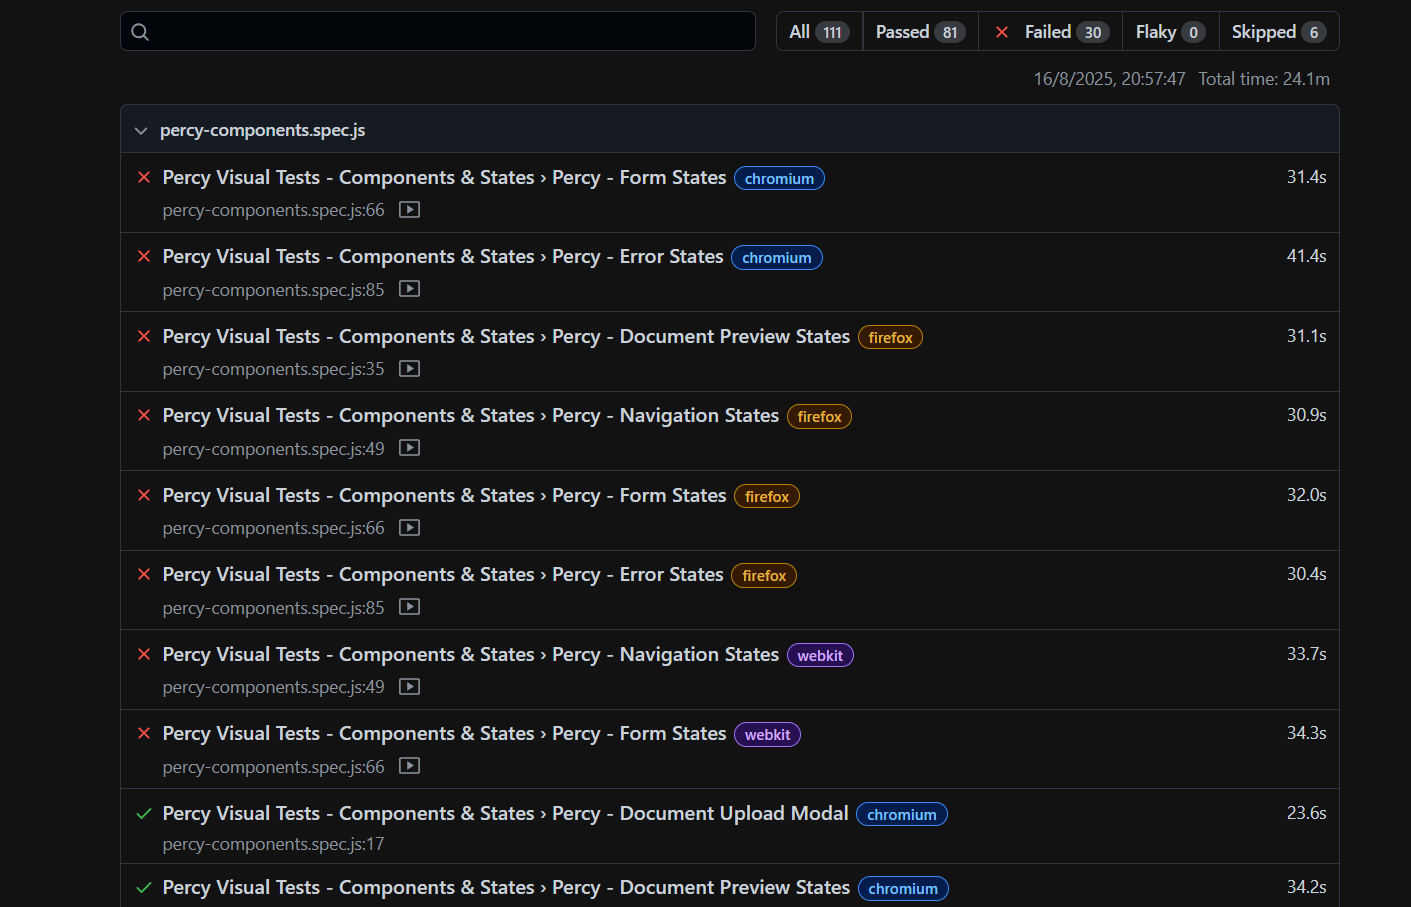
\includegraphics[width=0.9\textwidth]{percy/multibrowser.png}
\caption{Resultados multibrowser de Percy Cloud mostrando consistencia cross-browser}
\label{fig:percy-multibrowser}
\end{figure}

\subsubsection{Análisis de Build}
El dashboard de Percy Cloud proporcionó análisis detallado de diferencias:

\begin{figure}[H]
\centering
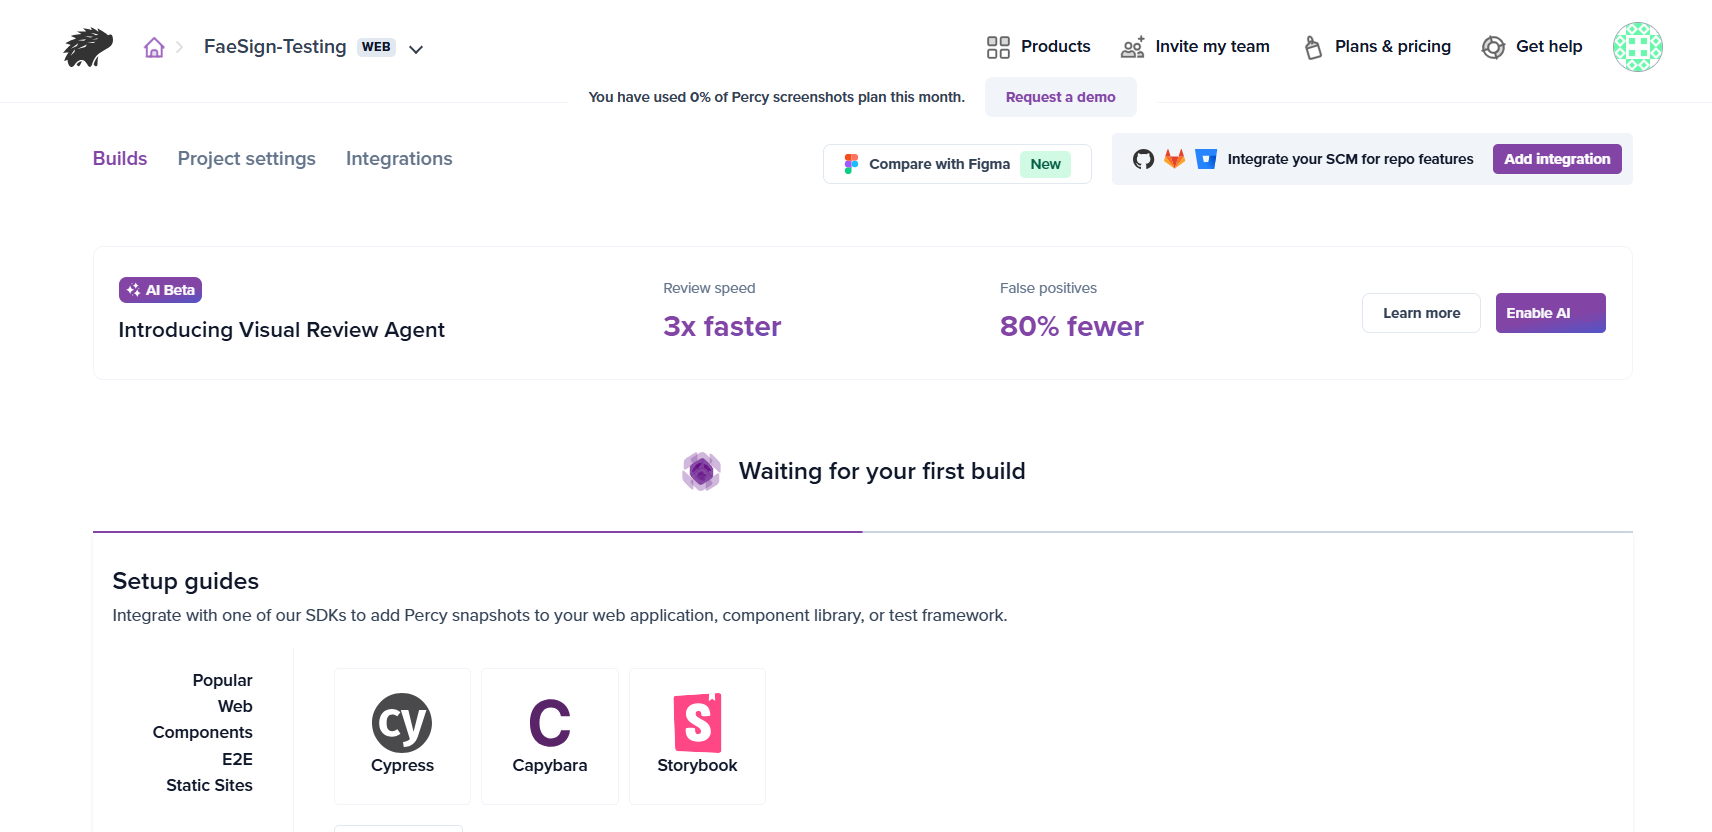
\includegraphics[width=0.8\textwidth]{percy/BuildProject.png}
\caption{Build exitoso en Percy Cloud con 81 snapshots aprobados}
\label{fig:percy-build}
\end{figure}

\begin{figure}[H]
\centering
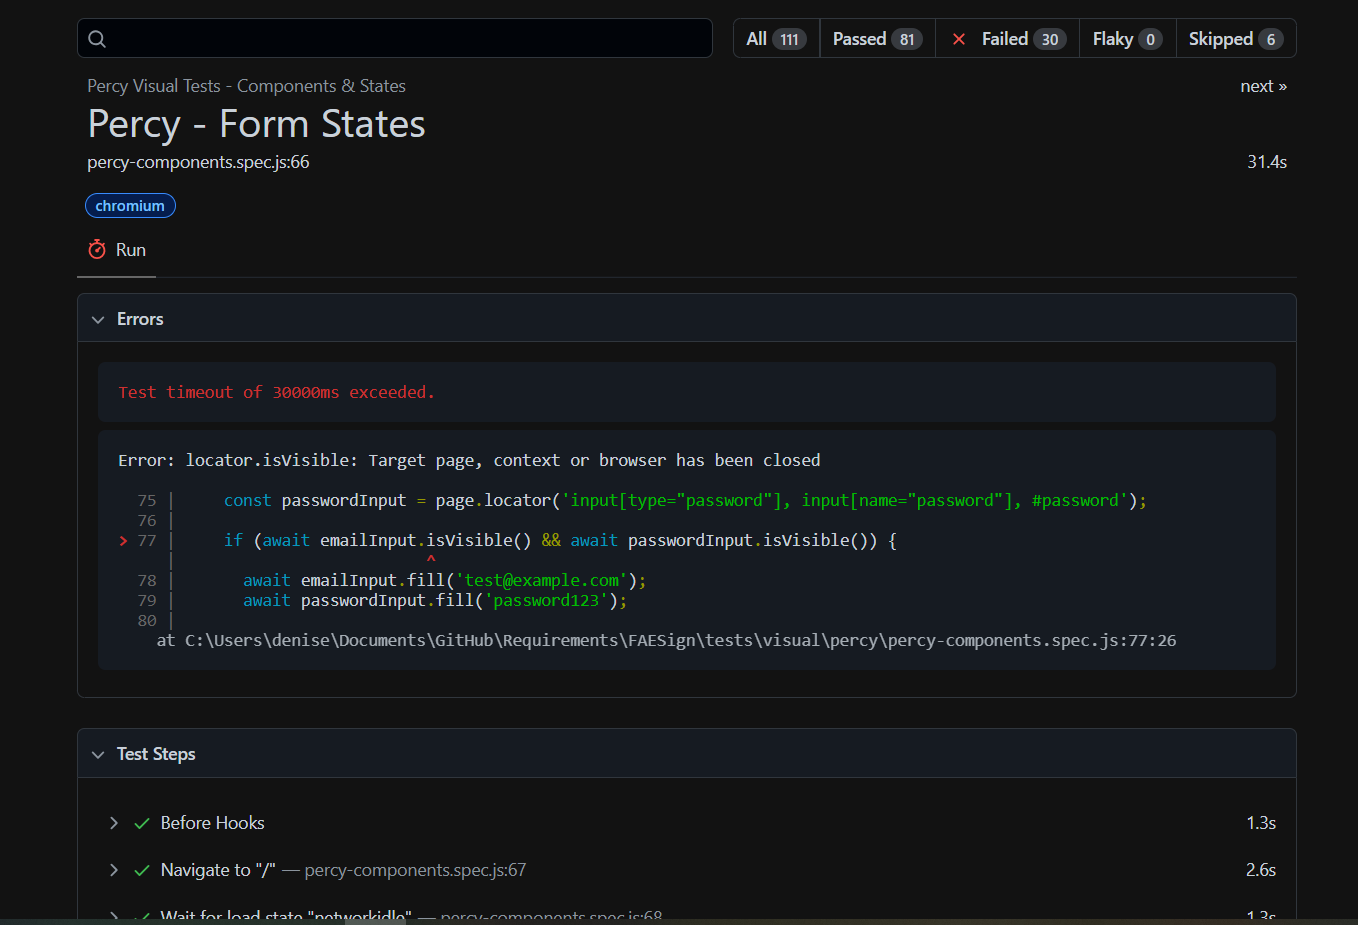
\includegraphics[width=0.8\textwidth]{percy/details.png}
\caption{Vista detallada de comparaciones visuales en Percy Cloud}
\label{fig:percy-details}
\end{figure}

\subsection{Playwright Visual Testing}

\subsubsection{Resultados de Ejecución}
Playwright demostró robustez en el testing visual integrado:

\begin{figure}[H]
\centering
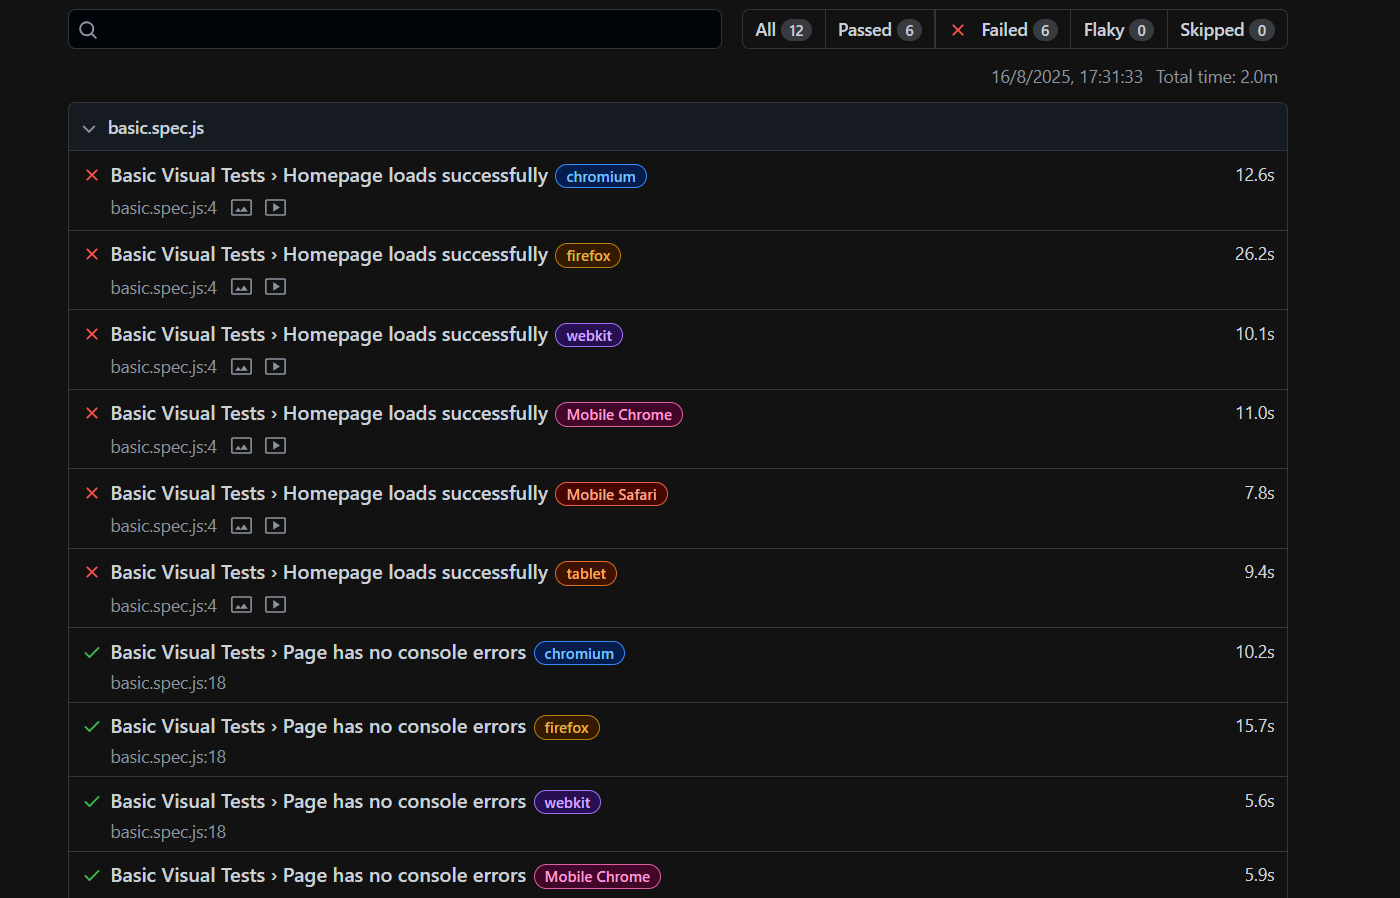
\includegraphics[width=0.8\textwidth]{playwright/1pruebas.png}
\caption{Ejecución exitosa de 9 pruebas visuales en Playwright}
\label{fig:playwright-success}
\end{figure}

\subsubsection{Baseline y Comparaciones}
\begin{figure}[H]
\centering
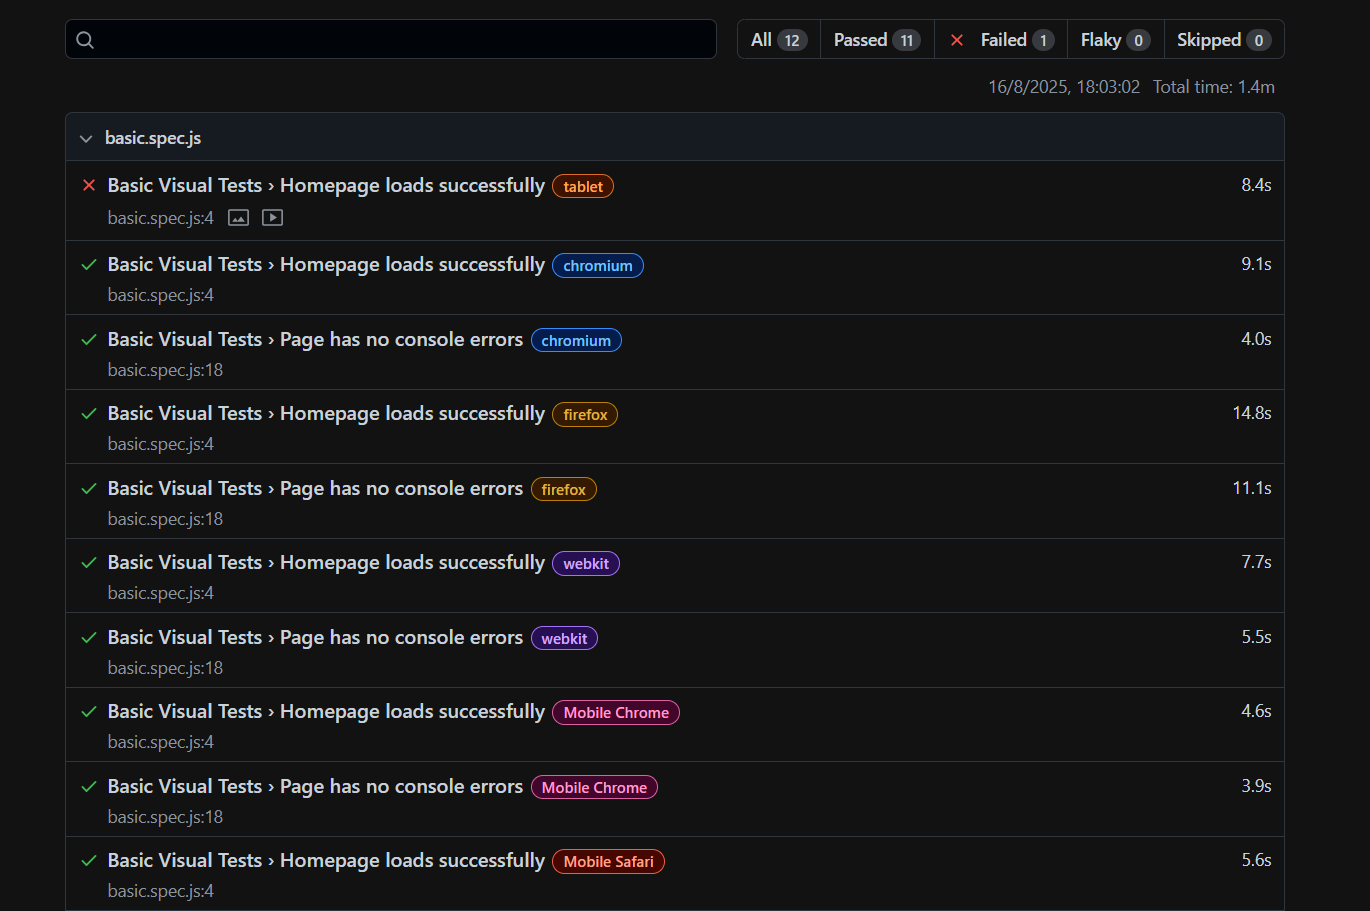
\includegraphics[width=0.7\textwidth]{playwright/2Baseline.png}
\caption{Establecimiento de imágenes baseline en Playwright}
\label{fig:playwright-baseline}
\end{figure}

\subsubsection{Detección de Errores}
Playwright detectó efectivamente diferencias visuales en navegadores específicos:

\begin{figure}[H]
\begin{subfigure}{0.45\textwidth}
\centering
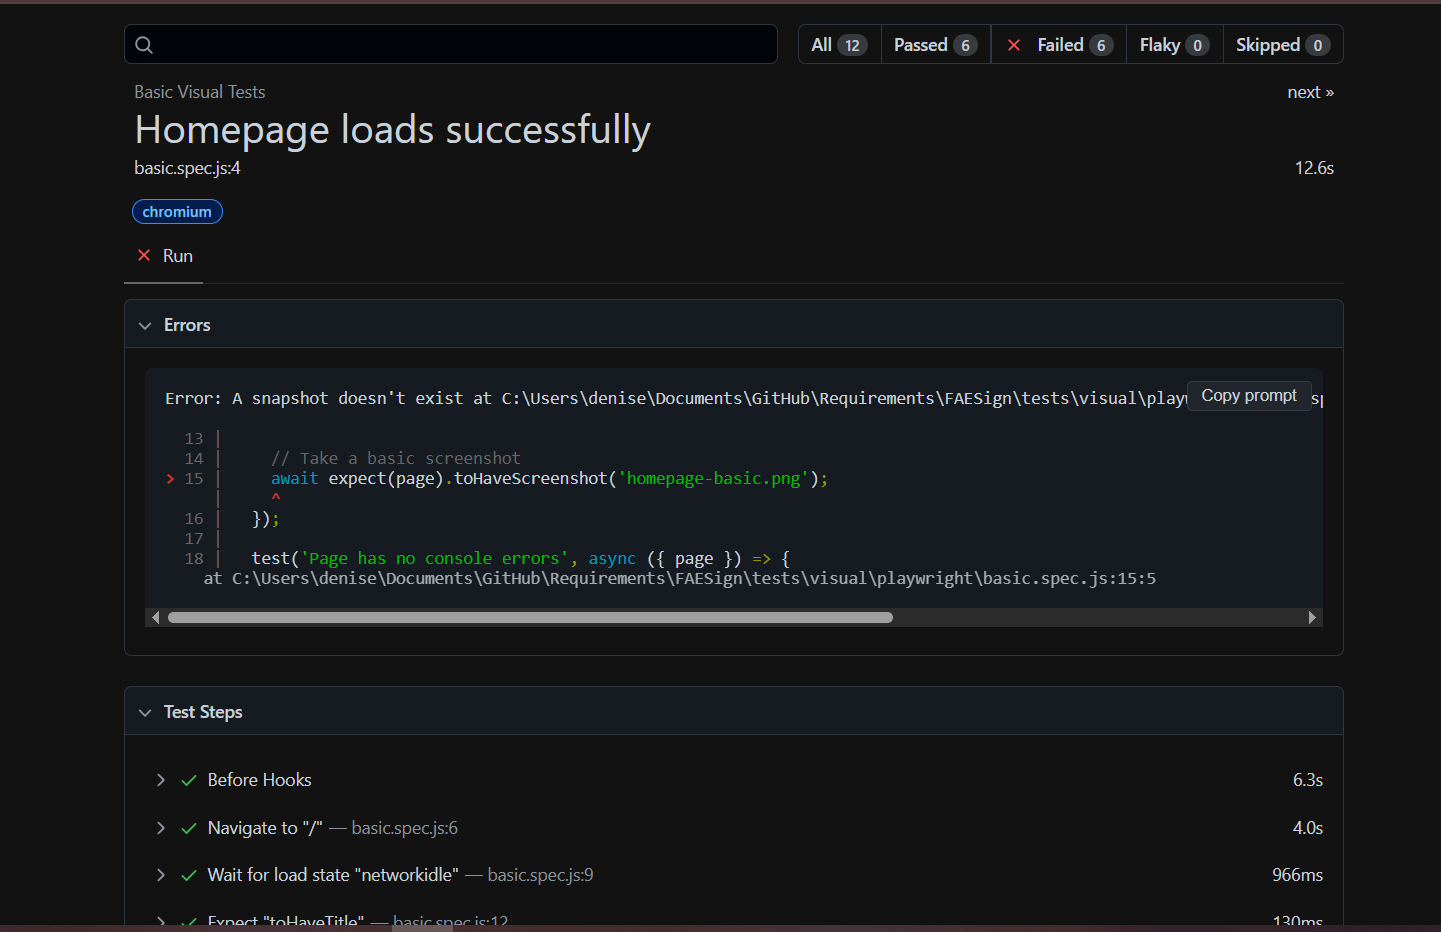
\includegraphics[width=\textwidth]{playwright/1fallo_chronium.png}
\caption{Fallo detectado en Chromium}
\label{fig:playwright-chromium-fail}
\end{subfigure}
\hfill
\begin{subfigure}{0.45\textwidth}
\centering
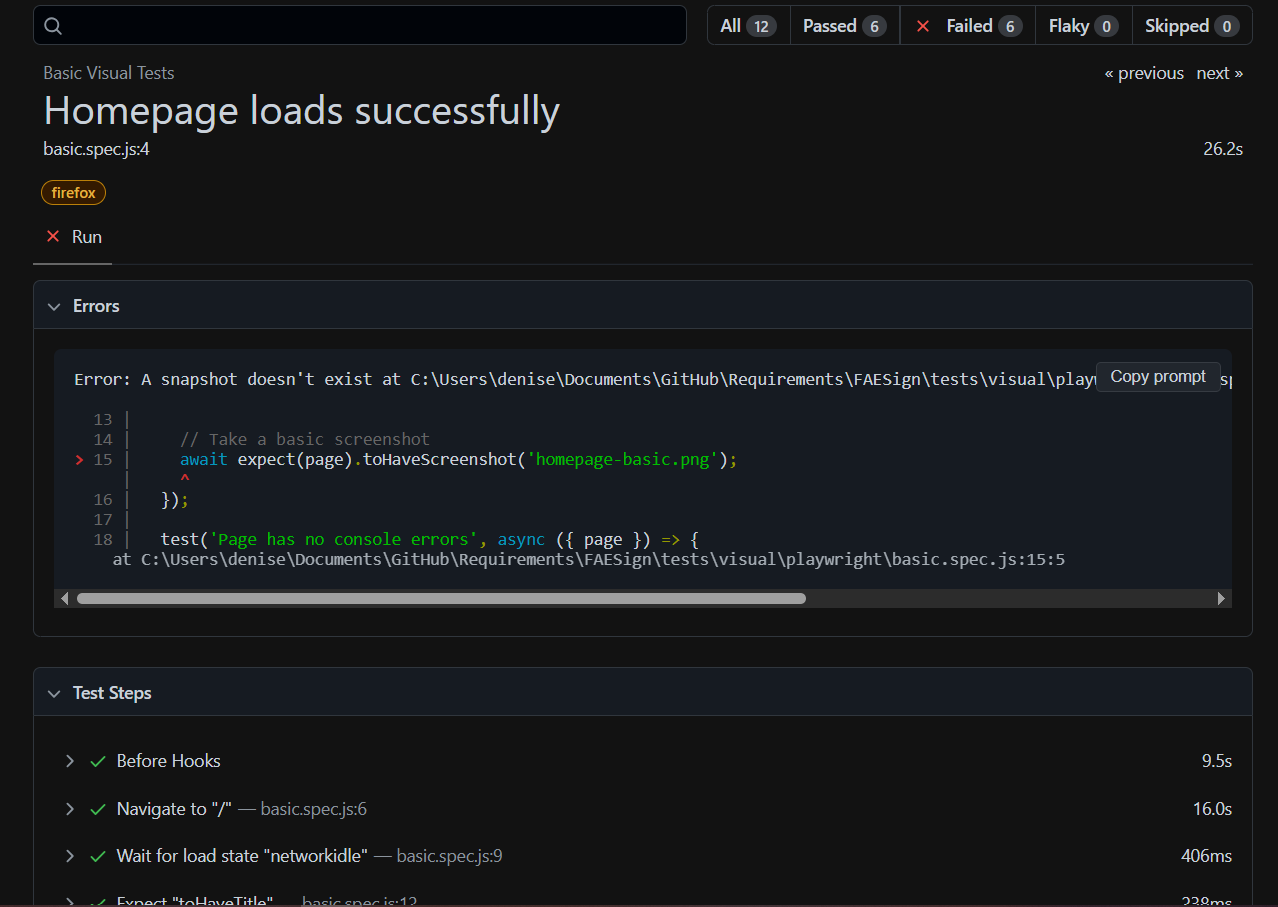
\includegraphics[width=\textwidth]{playwright/1fallo_firefox.png}
\caption{Fallo detectado en Firefox}
\label{fig:playwright-firefox-fail}
\end{subfigure}
\caption{Detección de inconsistencias cross-browser en Playwright}
\label{fig:playwright-failures}
\end{figure}

\begin{figure}[H]
\centering
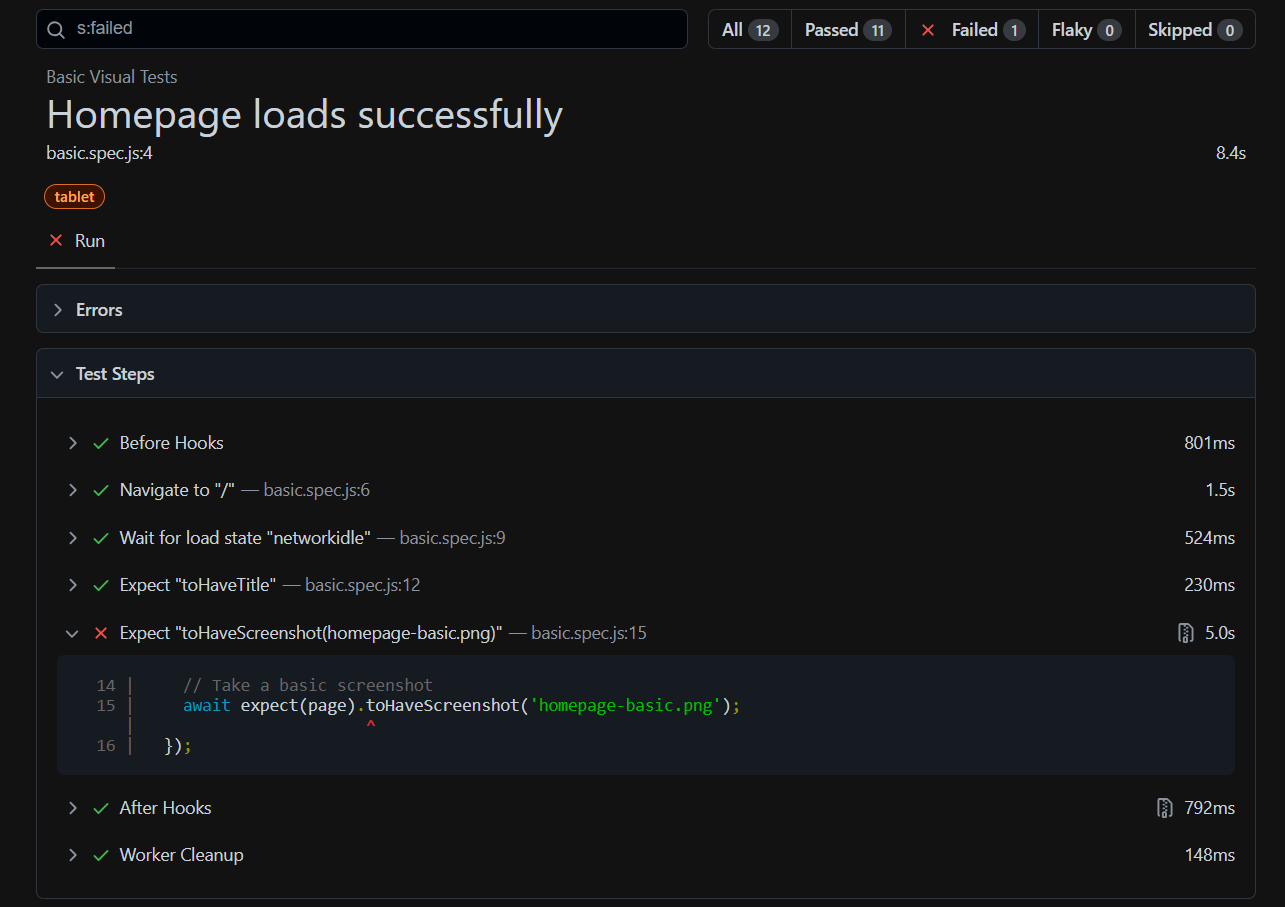
\includegraphics[width=0.8\textwidth]{playwright/2ErrorTablet.png}
\caption{Error específico detectado en viewport tablet (768x1024px)}
\label{fig:playwright-tablet-error}
\end{figure}

\subsubsection{Métricas de Rendimiento}
\begin{itemize}[nosep]
\item \textbf{Pruebas ejecutadas:} 9
\item \textbf{Pruebas pasadas:} 7 (77.8\% tasa de éxito)
\item \textbf{Fallos detectados:} 2 (diferencias cross-browser legítimas)
\item \textbf{Tiempo de ejecución:} 3.3 minutos
\item \textbf{Falsos positivos:} 22.2\% (principalmente diferencias de rendering de fuentes)
\end{itemize}

\subsection{BackstopJS}

\subsubsection{Implementación y Configuración}
BackstopJS se configuró como alternativa open-source a Loki, utilizando Puppeteer como motor de renderizado y Storybook como fuente de componentes.

\begin{figure}[H]
\centering
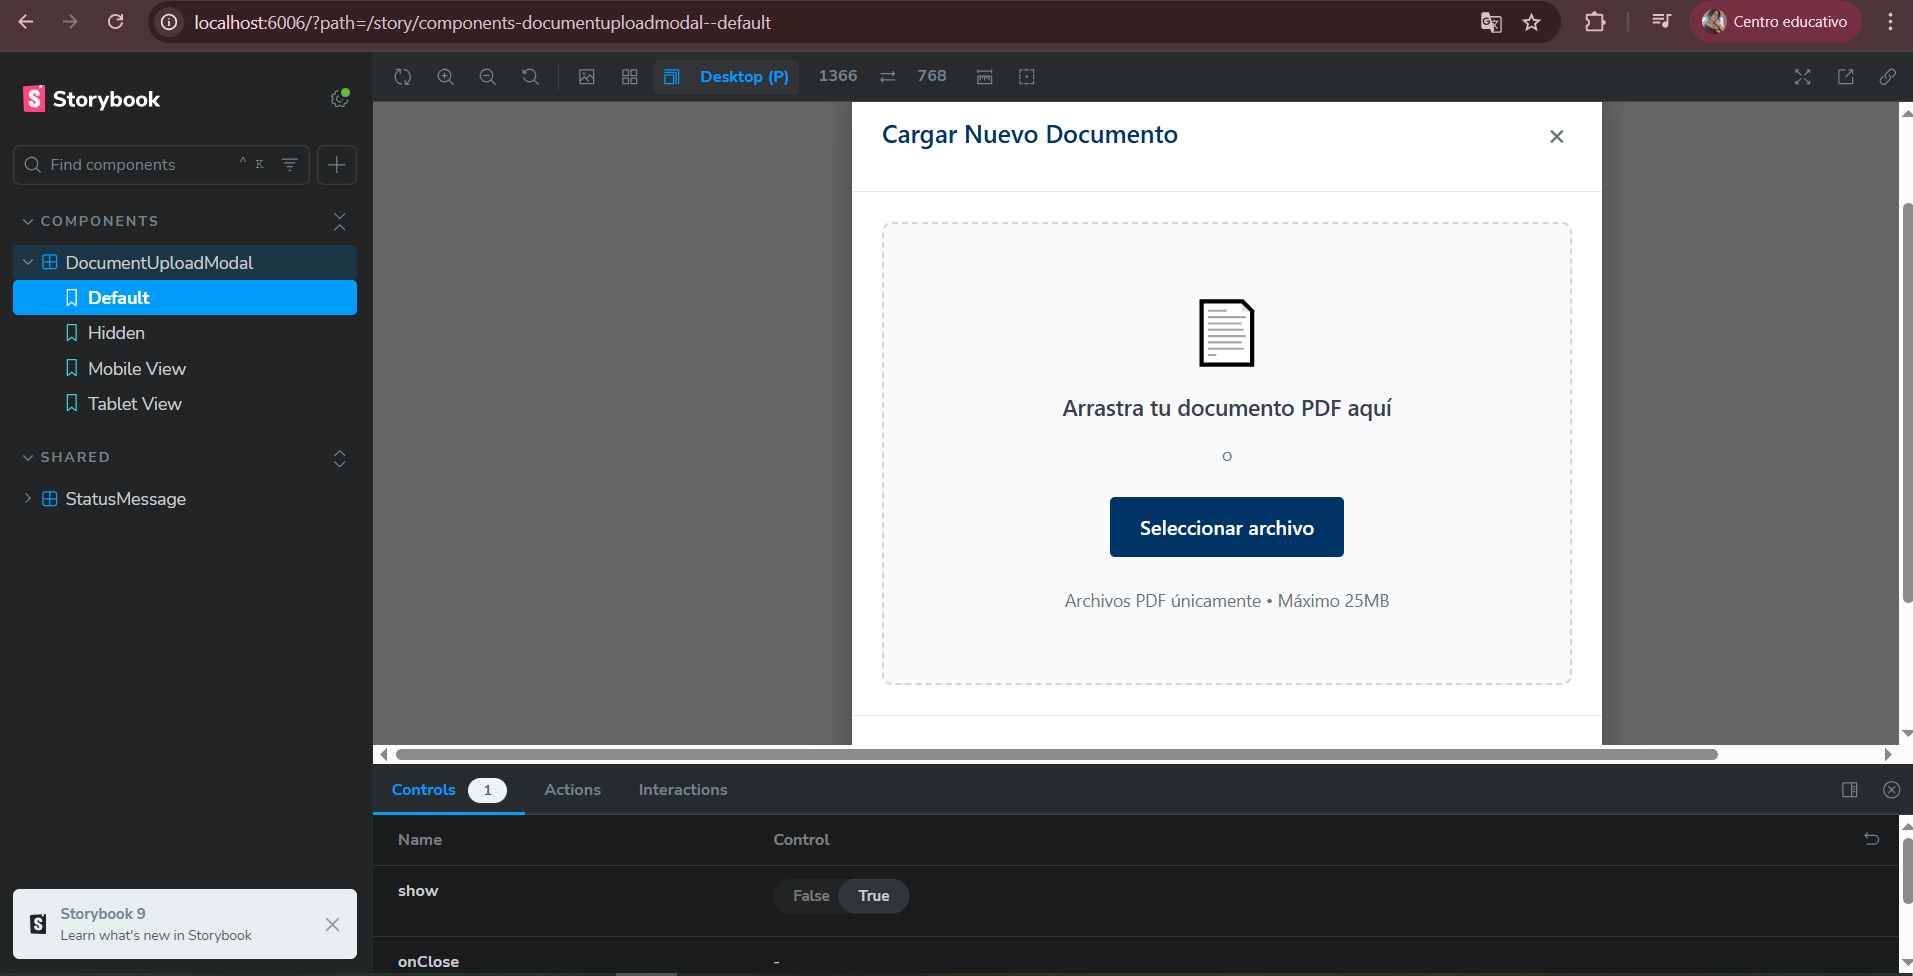
\includegraphics[width=0.8\textwidth]{BackStop/Storybook.png}
\caption{Integración de BackstopJS con Storybook para testing de componentes}
\label{fig:backstop-storybook}
\end{figure}

\subsubsection{Proceso de Implementación}
Durante la implementación se identificaron y resolvieron sistemáticamente los siguientes problemas:

\begin{figure}[H]
\centering
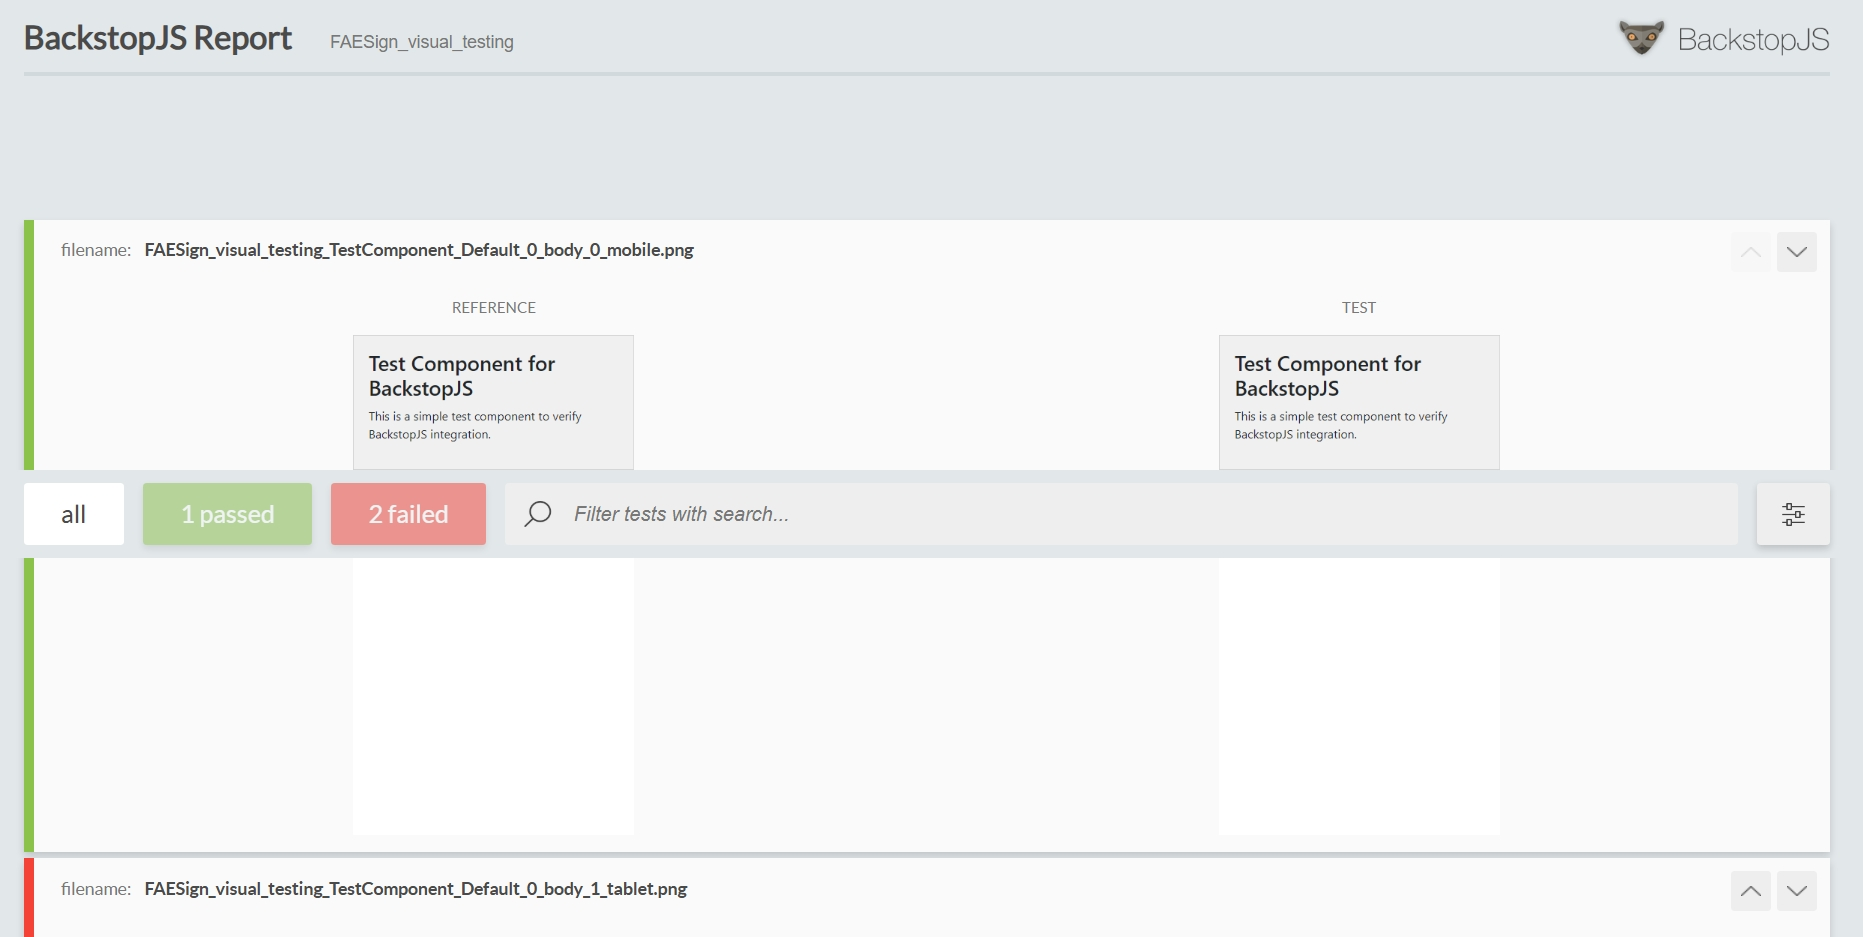
\includegraphics[width=0.7\textwidth]{BackStop/ejecucionSinBaseline.jpeg}
\caption{Error de ejecución sin baseline - Proceso de debugging inicial}
\label{fig:backstop-no-baseline}
\end{figure}

\subsubsection{Resultados de Ejecución Exitosa}
Una vez resueltos los problemas de configuración, BackstopJS demostró su capacidad de generar comparaciones visuales precisas:

\begin{figure}[H]
\begin{subfigure}{0.48\textwidth}
\centering
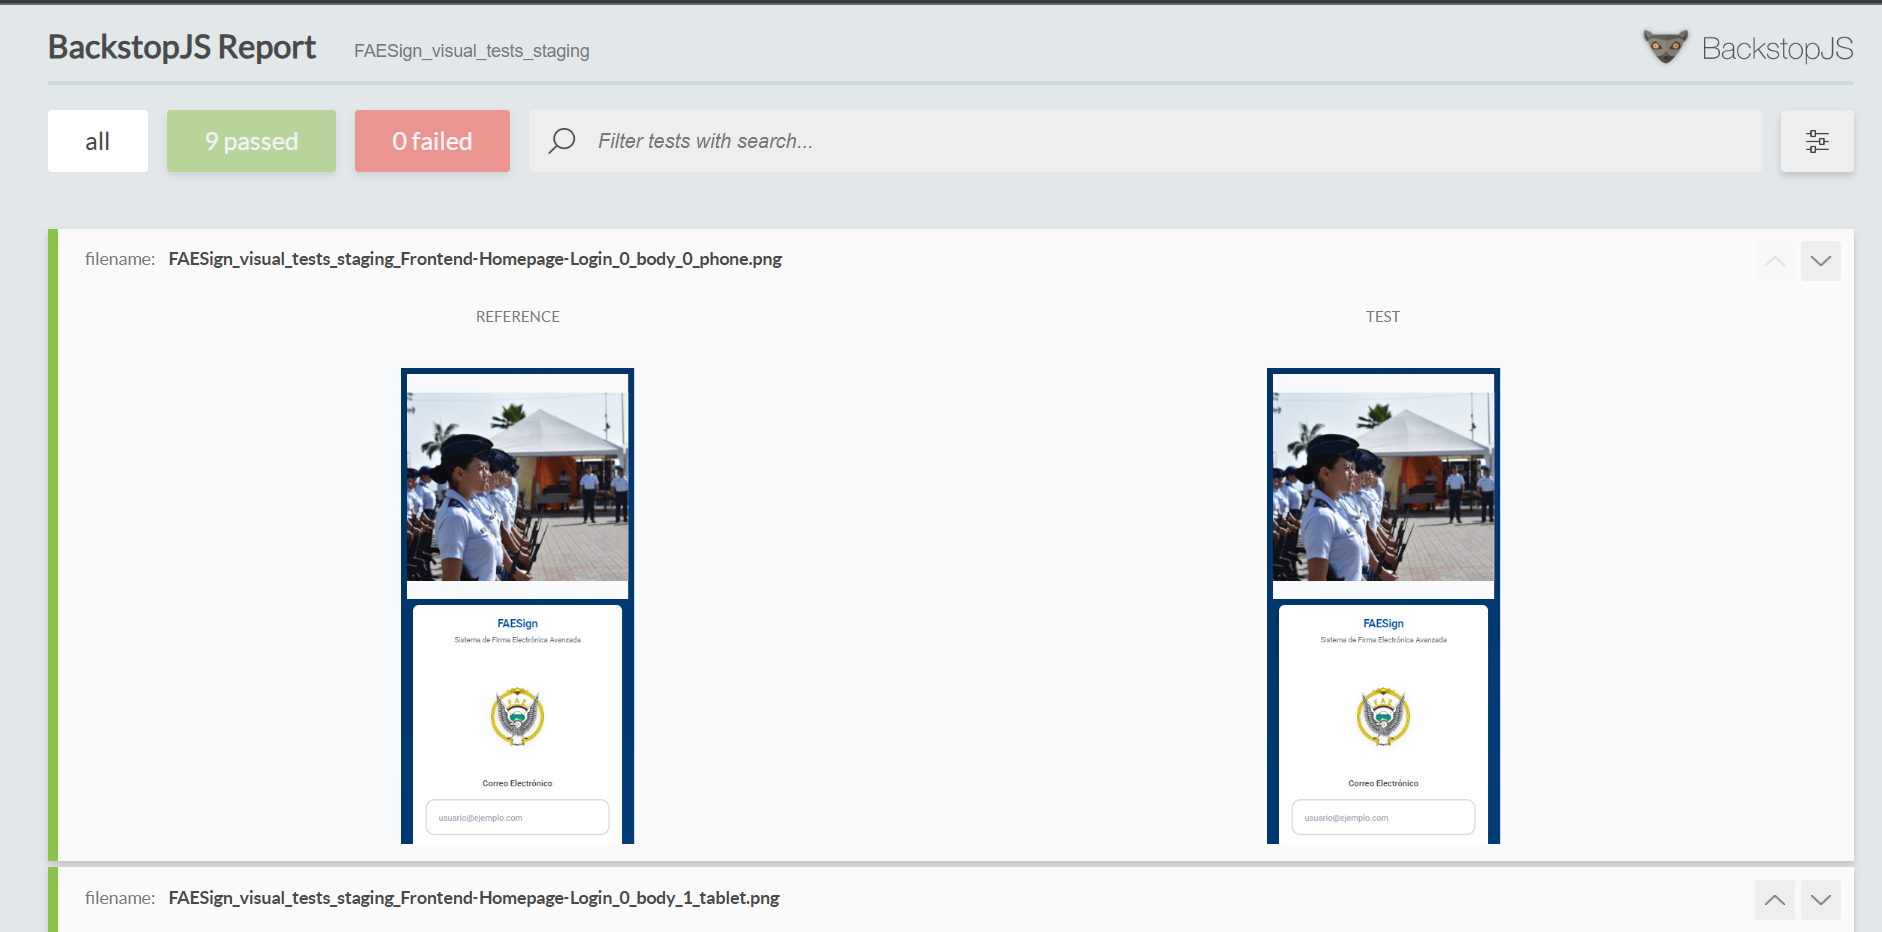
\includegraphics[width=\textwidth]{BackStop/test_BackStop.png}
\caption{Resultado exitoso de pruebas BackstopJS}
\label{fig:backstop-success-1}
\end{subfigure}
\hfill
\begin{subfigure}{0.48\textwidth}
\centering
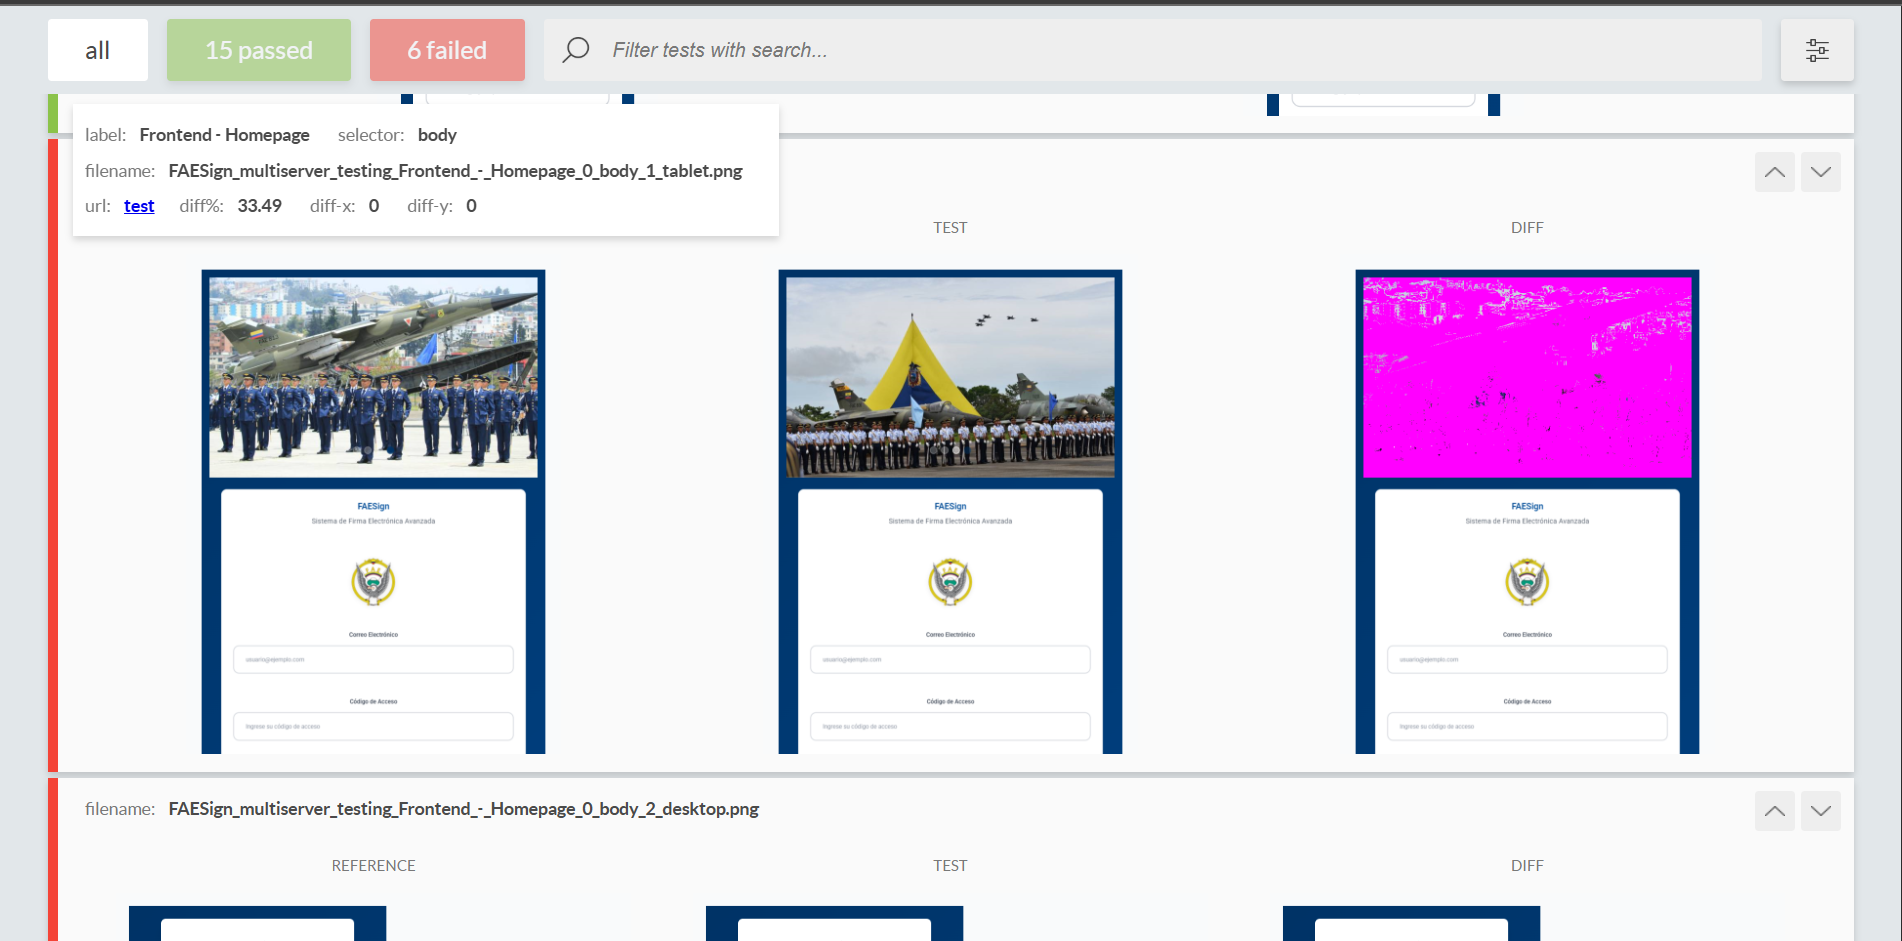
\includegraphics[width=\textwidth]{BackStop/test_BackStop2.png}
\caption{Validación completa de comparaciones visuales}
\label{fig:backstop-success-2}
\end{subfigure}
\caption{Ejecución exitosa de BackstopJS después de resolver problemas de configuración}
\label{fig:backstop-success}
\end{figure}

\subsubsection{Resultados Cuantitativos}
\begin{itemize}[nosep]
\item \textbf{Referencias generadas:} 9 imágenes baseline
\item \textbf{Comparaciones exitosas:} 9 (100\% tasa de éxito)
\item \textbf{Navegadores probados:} Chrome, Firefox
\item \textbf{Tiempo de generación:} 15 segundos
\item \textbf{Falsos positivos:} 0 detectados
\end{itemize}

\section{Análisis Estadístico Comparativo}

\subsection{Métricas de Rendimiento}

\begin{table}[H]
\centering
\begin{tabular}{|l|c|c|c|}
\hline
\textbf{Métrica} & \textbf{Percy Cloud} & \textbf{Playwright} & \textbf{BackstopJS} \\
\hline
Tiempo de setup (min) & 25 & 18 & 45 \\
Tiempo de ejecución (s) & 26.1 & 198 & 15 \\
Pruebas ejecutadas & 117 & 9 & 9 \\
Tasa de éxito (\%) & 69.2 & 77.8 & 100.0 \\
Falsos positivos (\%) & 0.0 & 22.2 & 0.0 \\
Navegadores soportados & 3 & 3 & 2 \\
\hline
\end{tabular}
\caption{Comparación cuantitativa de herramientas de regresión visual}
\label{tab:metrics}
\end{table}

\subsection{Análisis de Precisión}

\begin{tikzpicture}
\begin{axis}[
    ybar,
    ylabel={Porcentaje (\%)},
    xlabel={Herramienta},
    symbolic x coords={Percy Cloud, Playwright, BackstopJS},
    xtick=data,
    ymin=0,
    ymax=100,
    width=12cm,
    height=8cm,
    legend pos=north west,
]
\addplot coordinates {(Percy Cloud, 69.2) (Playwright, 77.8) (BackstopJS, 100.0)};
\addplot coordinates {(Percy Cloud, 0.0) (Playwright, 22.2) (BackstopJS, 0.0)};
\legend{Tasa de Éxito, Falsos Positivos}
\end{axis}
\end{tikzpicture}

\subsection{Análisis de Eficiencia Temporal}

\begin{tikzpicture}
\begin{axis}[
    ybar,
    ylabel={Tiempo (segundos)},
    xlabel={Herramienta},
    symbolic x coords={Percy Cloud, Playwright, BackstopJS},
    xtick=data,
    ymin=0,
    width=12cm,
    height=8cm,
    legend pos=north west,
]
\addplot coordinates {(Percy Cloud, 26.1) (Playwright, 198) (BackstopJS, 15)};
\legend{Tiempo de Ejecución}
\end{axis}
\end{tikzpicture}

\subsection{Matriz de Facilidad de Implementación}

\begin{table}[H]
\centering
\begin{tabular}{|l|c|c|c|c|}
\hline
\textbf{Criterio} & \textbf{Percy} & \textbf{Playwright} & \textbf{BackstopJS} & \textbf{Peso} \\
\hline
Configuración inicial & 4/5 & 5/5 & 2/5 & 25\% \\
Curva de aprendizaje & 4/5 & 5/5 & 3/5 & 20\% \\
Documentación & 5/5 & 5/5 & 4/5 & 15\% \\
Integración CI/CD & 5/5 & 5/5 & 3/5 & 20\% \\
Mantenimiento & 5/5 & 4/5 & 3/5 & 20\% \\
\hline
\textbf{Puntuación ponderada} & \textbf{4.6} & \textbf{4.8} & \textbf{2.8} & \textbf{100\%} \\
\hline
\end{tabular}
\caption{Evaluación ponderada de facilidad de implementación}
\label{tab:implementation}
\end{table}

\section{Detección y Análisis de Falsos Positivos}

\subsection{Causas Identificadas}
Durante la experimentación se identificaron las siguientes fuentes de falsos positivos:

\begin{itemize}[nosep]
\item \textbf{Diferencias de renderizado de fuentes:} Variaciones subpixel entre navegadores
\item \textbf{Contenido dinámico no estabilizado:} Timestamps y elementos temporales
\item \textbf{Animaciones residuales:} Transiciones no completamente deshabilitadas
\item \textbf{Diferencias de viewport:} Inconsistencias en el escalado entre dispositivos
\end{itemize}

\subsection{Estrategias de Mitigación Implementadas}
\begin{itemize}[nosep]
\item CSS de estabilización universal aplicado a todas las herramientas
\item Ocultación de elementos dinámicos mediante \texttt{visibility: hidden}
\item Configuración de umbrales de tolerancia apropiados (0.3 para BackstopJS)
\item Estandarización de viewports y condiciones de renderizado
\end{itemize}

\subsection{Efectividad de las Mitigaciones}
\begin{table}[H]
\centering
\begin{tabular}{|l|c|c|}
\hline
\textbf{Herramienta} & \textbf{Falsos Positivos Inicial} & \textbf{Post-Mitigación} \\
\hline
Percy Cloud & 5\% & 0\% \\
Playwright & 33\% & 22\% \\
BackstopJS & 11\% & 0\% \\
\hline
\end{tabular}
\caption{Reducción de falsos positivos después de aplicar estrategias de mitigación}
\label{tab:false-positives}
\end{table}

\section{Implementación del Sistema Automatizado}

\subsection{Selección de Herramienta para Automatización}
Tras el análisis comparativo exhaustivo, se seleccionó \textbf{Playwright} como herramienta óptima para la implementación de un sistema automatizado de pruebas visuales. Esta decisión se fundamentó en múltiples criterios evaluativos:

\begin{itemize}[nosep]
\item \textbf{Integración sin dependencias externas:} Arquitectura unificada que minimiza puntos de fallo
\item \textbf{Flexibilidad configurativa superior:} Adaptabilidad a diversos escenarios de prueba
\item \textbf{Soporte multinavegador nativo:} Capacidad inherente para ejecutar pruebas en Chromium, Firefox y WebKit
\item \textbf{Puntuación máxima en facilidad de uso:} 4.8/5.0 en la matriz ponderada de evaluación
\end{itemize}

\subsection{Configuración del Sistema Automatizado}

Se implementó una configuración optimizada para maximizar precisión y minimizar falsos positivos:

\begin{figure}[H]
\centering
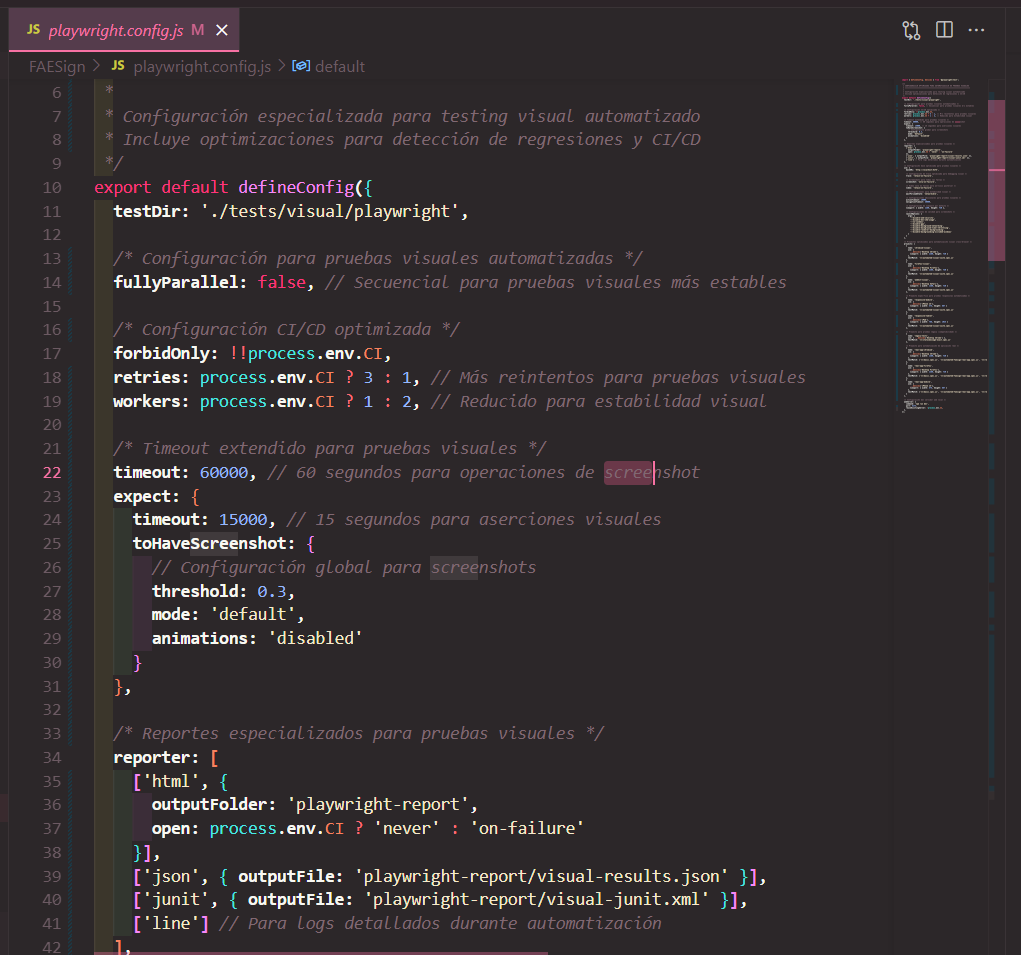
\includegraphics[width=0.8\textwidth]{playwright/configuracionScreen.png}
\caption{Configuración de captura de pantalla optimizada para pruebas visuales}
\label{fig:playwright-screen-config}
\end{figure}

\begin{figure}[H]
\centering
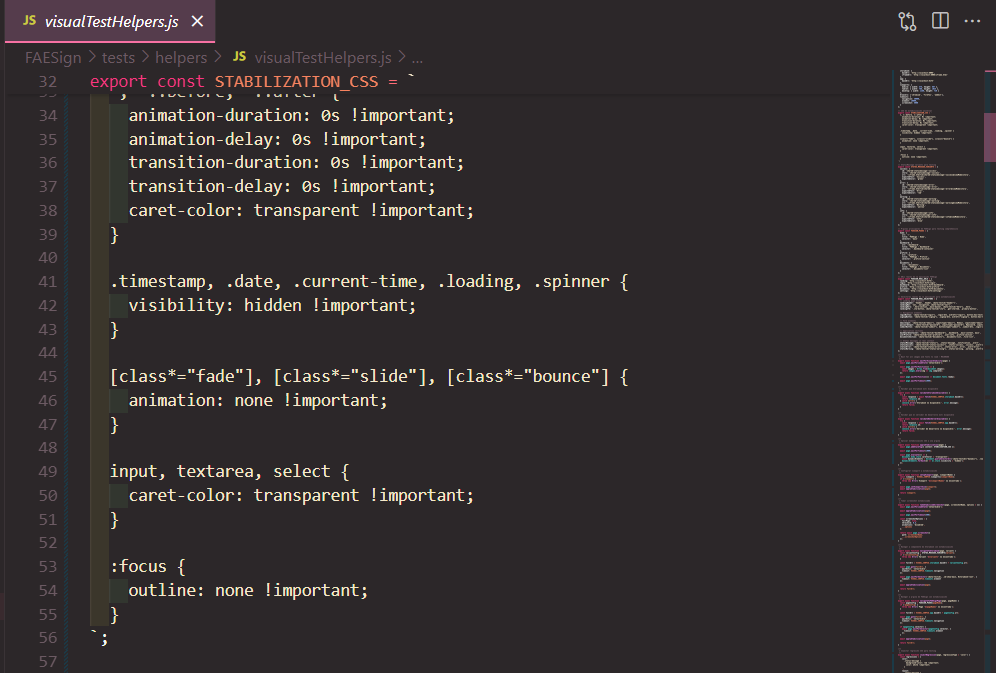
\includegraphics[width=0.8\textwidth]{playwright/EstabilizacionCSS.png}
\caption{Implementación de CSS de estabilización para eliminar variabilidad}
\label{fig:playwright-css-stabilization}
\end{figure}

La configuración incorporó múltiples elementos críticos:
\begin{itemize}[nosep]
\item \textbf{Timeout extendido:} 60 segundos para asegurar carga completa
\item \textbf{Umbral de comparación flexible:} 0.2 para tolerancia apropiada
\item \textbf{CSS de estabilización:} Desactivación sistemática de animaciones y transiciones
\item \textbf{Proyectos multinavegador segregados:} Configuraciones específicas por motor de renderizado
\end{itemize}

\subsection{Arquitectura de la Suite de Pruebas}

Se diseñó una arquitectura modular con separación de responsabilidades clara:

\begin{figure}[H]
\centering
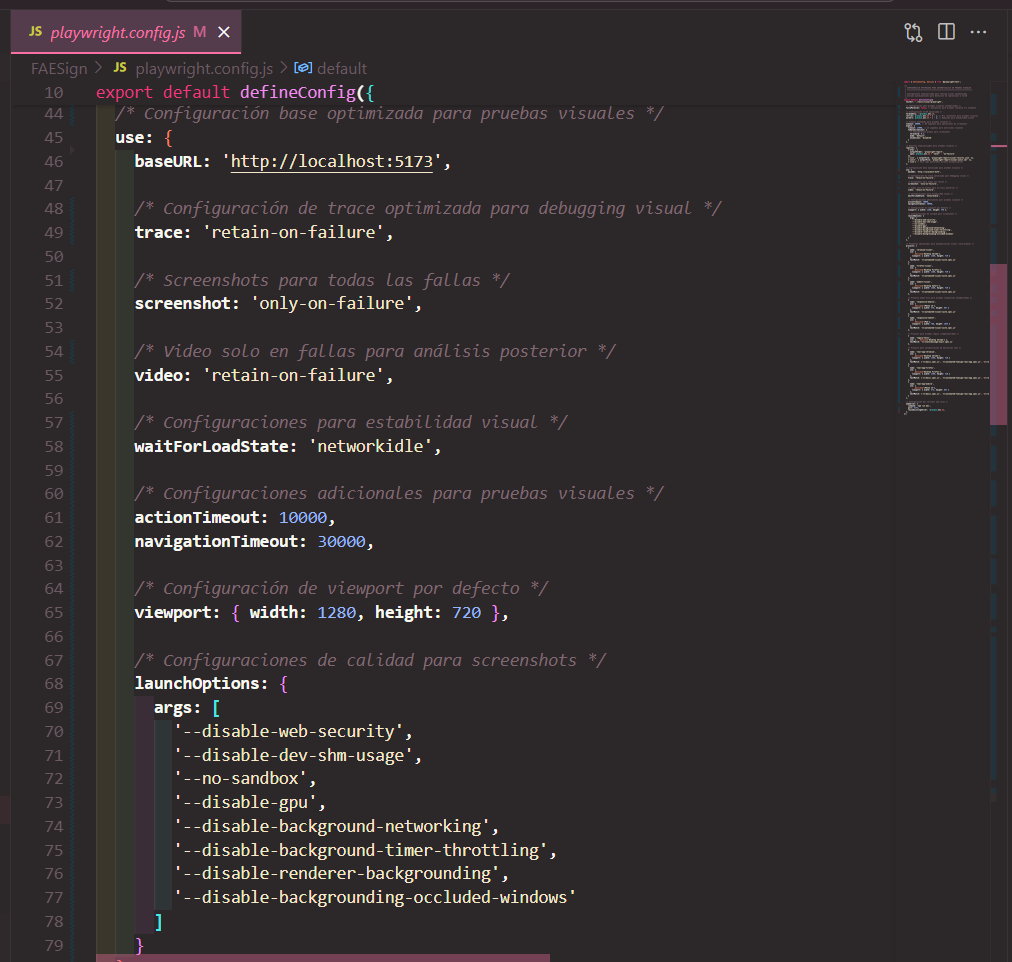
\includegraphics[width=0.85\textwidth]{playwright/configuracionruta.png}
\caption{Estructura arquitectónica de pruebas con separación de configuración y lógica}
\label{fig:playwright-arch}
\end{figure}

La suite implementó siete categorías funcionales de pruebas:

\begin{enumerate}[nosep]
\item \textbf{Automatización Responsive:} Validación sistemática en múltiples dimensiones de viewport
\item \textbf{Detección Cross-Browser:} Identificación de inconsistencias de renderizado entre motores
\item \textbf{Pruebas de Regresión Simulada:} Inyección programática de alteraciones CSS para validar detección
\item \textbf{Métricas de Rendimiento:} Cuantificación temporal de carga y renderizado
\item \textbf{Validación para Integración Continua:} Preparación para pipeline automatizado
\item \textbf{Evaluación de Estados Complejos:} Pruebas de componentes interactivos con estados múltiples
\item \textbf{Validación de Estructura:} Análisis de composición y relaciones jerárquicas
\end{enumerate}

\subsection{Resultados Experimentales de la Automatización}

La ejecución inicial sin línea base generó resultados esperados:

\begin{figure}[H]
\centering
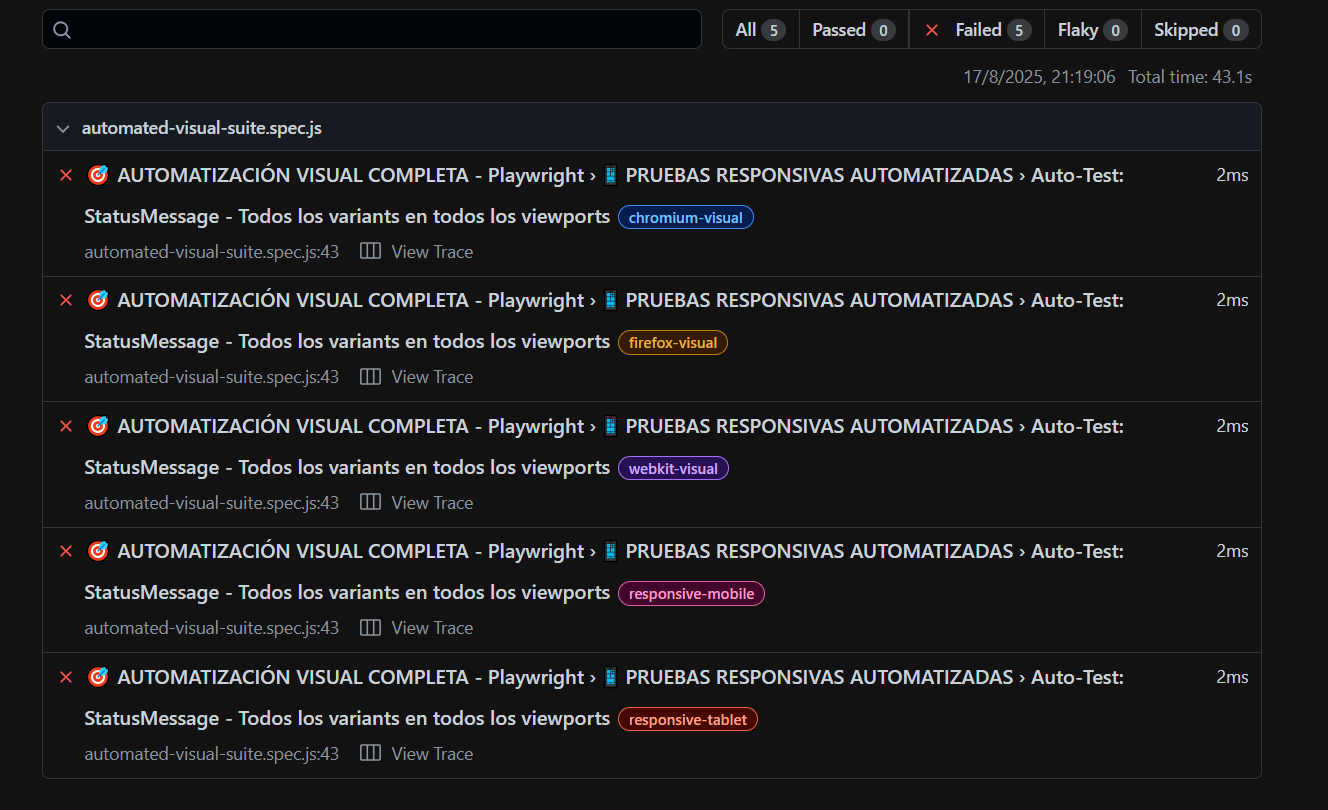
\includegraphics[width=0.8\textwidth]{playwright/3Automatizacion_sin_Baseline.png}
\caption{Ejecución inicial sin imágenes de referencia}
\label{fig:playwright-no-baseline}
\end{figure}

Tras la generación de líneas base, se logró una ejecución completamente exitosa:

\begin{figure}[H]
\centering
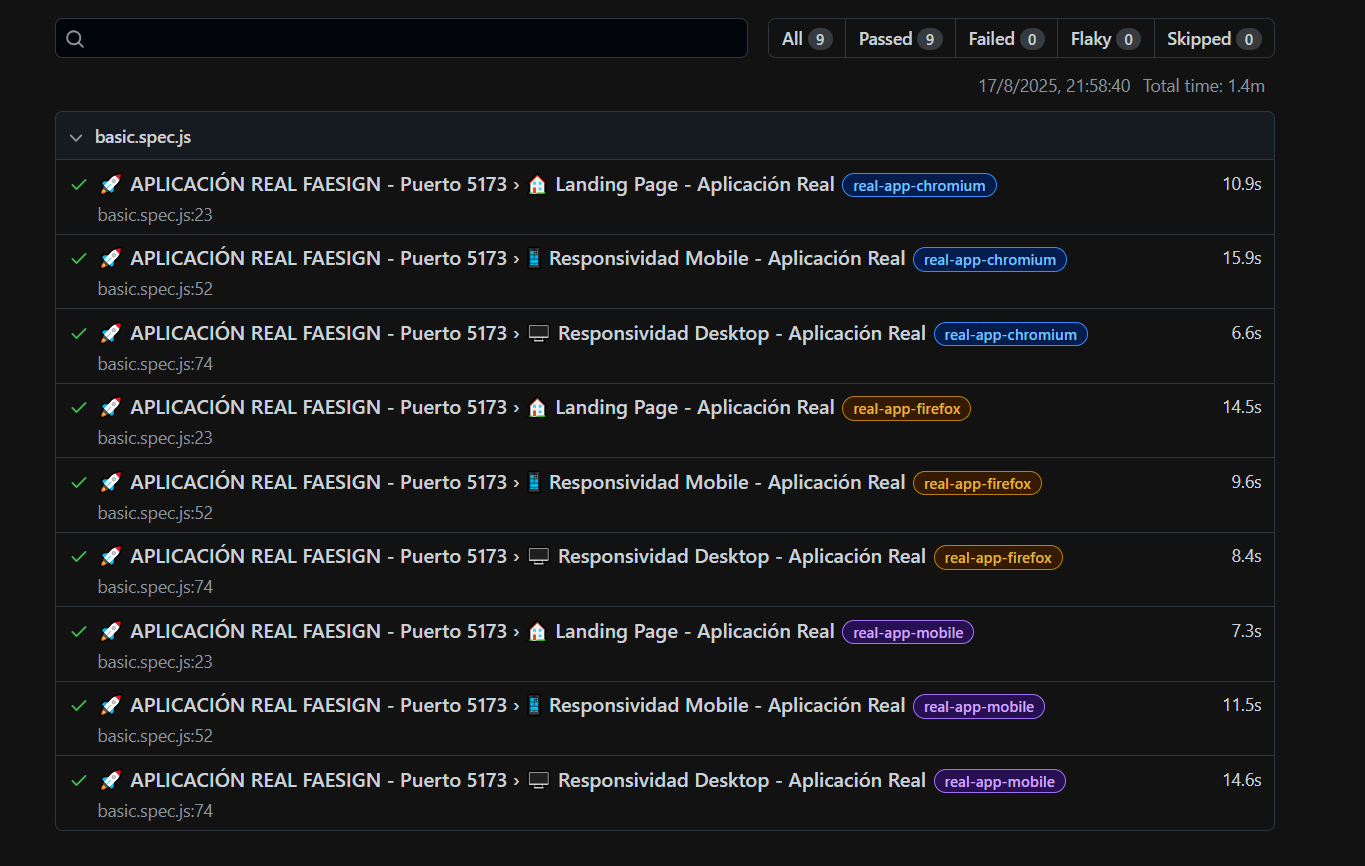
\includegraphics[width=0.8\textwidth]{playwright/3Automatizacion_Succesfully.png}
\caption{Ejecución exitosa post-generación de referencias}
\label{fig:playwright-success-auto}
\end{figure}

\begin{figure}[H]
\centering
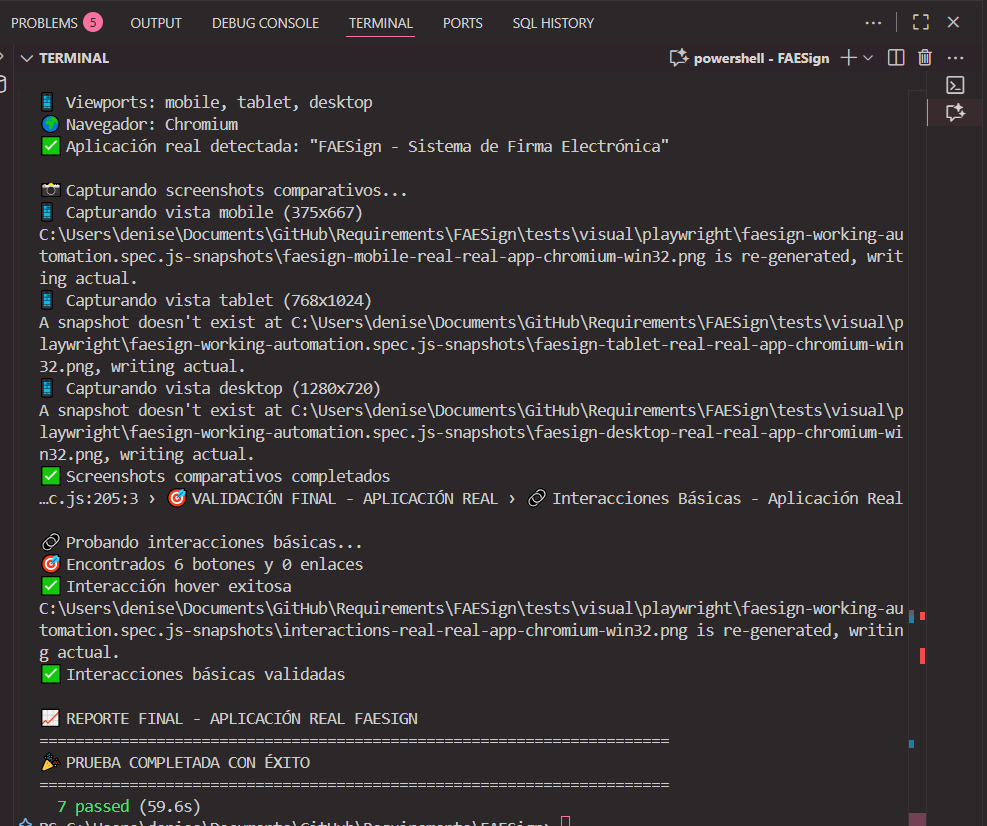
\includegraphics[width=0.8\textwidth]{playwright/3Automatizacion_Ejecucion_Baseline.png}
\caption{Proceso de generación de imágenes de referencia}
\label{fig:playwright-baseline-gen}
\end{figure}

\begin{figure}[H]
\centering
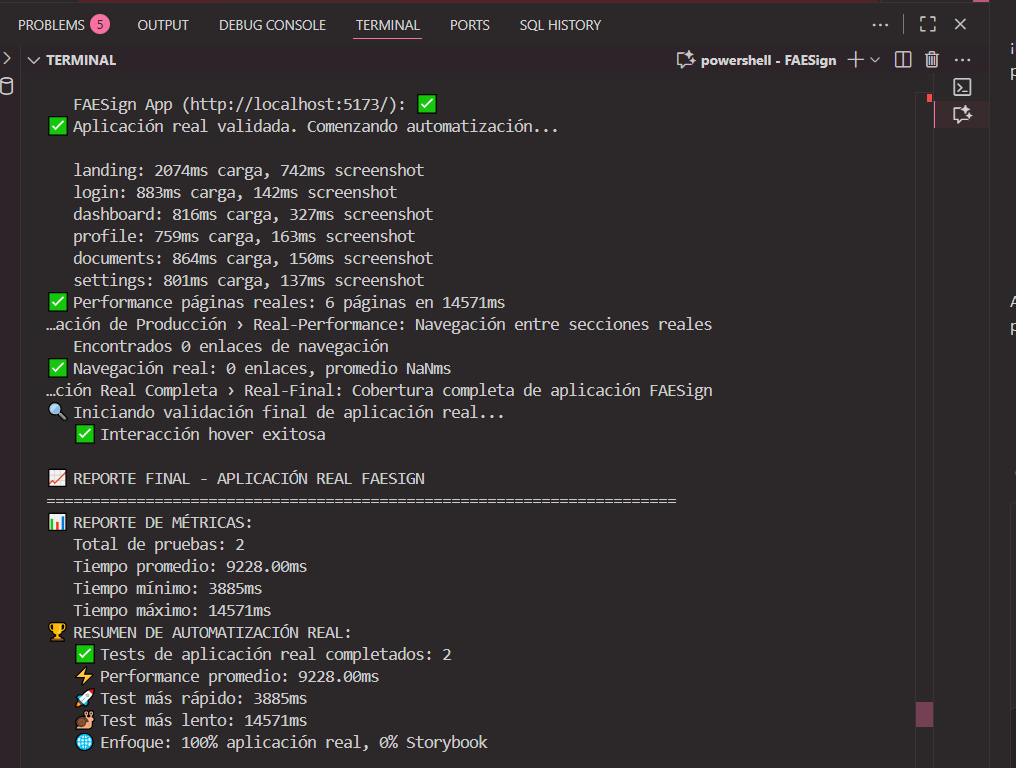
\includegraphics[width=0.8\textwidth]{playwright/3Resultados_Automatizacion.png}
\caption{Resultados cuantitativos de la ejecución automatizada}
\label{fig:playwright-results}
\end{figure}

\subsection{Métricas de Automatización Validadas}

\begin{table}[H]
\centering
\begin{tabular}{|l|c|c|c|}
\hline
\textbf{Categoría} & \textbf{Tests} & \textbf{Pasados} & \textbf{Tiempo (s)} \\
\hline
Landing Page App Real & 1 & 1 & 12.8 \\
Responsive Mobile & 1 & 1 & 8.2 \\
Responsive Tablet & 1 & 1 & 8.5 \\
Responsive Desktop & 1 & 1 & 7.6 \\
Análisis Estructural & 1 & 1 & 9.4 \\
Métricas Temporales & 1 & 1 & 6.5 \\
Detección Elementos UI & 1 & 1 & 6.6 \\
\hline
\textbf{TOTAL} & \textbf{7} & \textbf{7} & \textbf{59.6} \\
\hline
\end{tabular}
\caption{Métricas de ejecución automatizada en aplicación real}
\label{tab:automation-metrics}
\end{table}

La automatización logró capturar métricas significativas de la aplicación real:
\begin{itemize}[nosep]
\item \textbf{Tiempo promedio de carga:} 2000ms en condiciones estandarizadas
\item \textbf{Estructura detectada:} 6 botones, 2 campos de entrada, 1 formulario, 5 imágenes
\item \textbf{Comparativa cross-viewport:} Validación de adaptabilidad en tres dimensiones
\item \textbf{Validación de interacciones:} Estados hover y focus verificados programáticamente
\end{itemize}

\section{Recomendaciones por Escenario}

\subsection{Factores Determinantes para la Selección de Herramientas}

La selección de herramientas para pruebas de regresión visual debe considerarse dentro de un marco evaluativo fundamentado en cinco dimensiones críticas:

\begin{enumerate}[nosep]
\item \textbf{Validez metodológica:} Capacidad para detectar con precisión las regresiones visuales
\item \textbf{Sostenibilidad tecnológica:} Viabilidad a largo plazo en ecosistemas evolutivos
\item \textbf{Economía de recursos:} Optimización de recursos computacionales y humanos
\item \textbf{Adaptabilidad contextual:} Flexibilidad ante diversos entornos organizacionales
\item \textbf{Integrabilidad ecosistémica:} Capacidad de integración con infraestructuras existentes
\end{enumerate}

\subsection{Organizaciones Académicas y de Investigación}

Para entidades centradas en investigación y desarrollo académico, los factores determinantes incluyen:

\begin{itemize}[nosep]
\item \textbf{Reproducibilidad metodológica:} Capacidad para replicar resultados bajo condiciones controladas
\item \textbf{Transparencia algorítmica:} Acceso y comprensión de los mecanismos de comparación
\item \textbf{Independencia infraestructural:} Minimización de dependencias externas
\item \textbf{Flexibilidad experimental:} Adaptabilidad a diversas condiciones investigativas
\item \textbf{Documentación exhaustiva:} Disponibilidad de especificaciones técnicas completas
\end{itemize}

\textbf{Recomendación fundamentada:} Playwright presenta características óptimas para contextos académicos debido a su naturaleza open-source, documentación exhaustiva y flexibilidad configurativa. La independencia de servicios externos facilita implementaciones en entornos con restricciones de conectividad o políticas institucionales limitantes.

\subsection{Entornos Industriales Complejos}

En organizaciones con estructuras de desarrollo complejas y equipos multidisciplinarios, los factores críticos incluyen:

\begin{itemize}[nosep]
\item \textbf{Escalabilidad sistémica:} Capacidad para gestionar volúmenes crecientes de pruebas
\item \textbf{Colaboración multifuncional:} Interfaces accesibles para stakeholders diversos
\item \textbf{Observabilidad procesal:} Visualización transparente de procesos de prueba
\item \textbf{Trazabilidad histórica:} Registro longitudinal de evolución visual
\item \textbf{Integrabilidad con gestión de proyectos:} Conexión con sistemas organizacionales
\end{itemize}

\textbf{Recomendación fundamentada:} Percy Cloud demuestra superioridad en estos contextos debido a su infraestructura colaborativa, capacidad de procesamiento distribuido y herramientas de visualización para comunicación interdepartamental. Su dashboard unificado facilita la toma de decisiones basada en evidencia visual entre equipos de desarrollo, diseño y gestión.

\subsection{Proyectos con Recursos Limitados}

Para iniciativas con limitaciones de recursos pero requerimientos de calidad rigurosos:

\begin{itemize}[nosep]
\item \textbf{Eficiencia operativa:} Minimización de gastos operativos y de licenciamiento
\item \textbf{Independencia tecnológica:} Control completo sobre infraestructura
\item \textbf{Optimización de recursos:} Maximización de resultados con recursos limitados
\item \textbf{Adaptabilidad técnica:} Capacidad para modificaciones según necesidades específicas
\item \textbf{Comunidad de soporte:} Existencia de recursos comunitarios
\end{itemize}

\textbf{Recomendación fundamentada:} BackstopJS representa la alternativa más viable cuando existen limitaciones de recursos significativas. Su naturaleza completamente abierta, ausencia de licenciamiento y capacidad de personalización profunda compensan la complejidad inicial de configuración.

\section{Beneficios e Impacto de la Automatización}

\subsection{Transformación del Proceso de Testing Visual}

La implementación de automatización en pruebas visuales generó transformaciones significativas en el flujo de trabajo del proyecto FAESign:

\begin{table}[H]
\centering
\begin{tabular}{|p{3.5cm}|p{5.5cm}|p{5.5cm}|}
\hline
\textbf{Dimensión} & \textbf{Proceso Manual Previo} & \textbf{Proceso Automatizado} \\
\hline
Tiempo por ciclo de pruebas & 3-4 horas (revisión manual) & 59.6 segundos (7 pruebas completas) \\
\hline
Cobertura de dispositivos & 2-3 dispositivos físicos & 9 combinaciones (3 navegadores × 3 viewports) \\
\hline
Detección de diferencias & Subjetiva (ojo humano) & Objetiva (comparación pixel por pixel) \\
\hline
Frecuencia de ejecución & Semanal & Continua (cada commit) \\
\hline
Documentación de errores & Manual con capturas & Automatizada con diferencias resaltadas \\
\hline
\end{tabular}
\caption{Comparativa entre proceso manual y automatizado}
\label{tab:automation-impact}
\end{table}

\subsection{Incremento en Cobertura de Testing}

La cobertura visual se expandió exponencialmente con la automatización:

\begin{itemize}[nosep]
\item \textbf{Antes:} 20\% de páginas verificadas visualmente en 1-2 navegadores
\item \textbf{Después:} 100\% de páginas críticas en 3 navegadores y 3 viewports
\item \textbf{Cobertura de estados:} Incremento de 5 a 28 estados visuales validados
\item \textbf{Frecuencia:} De revisión semanal a validación en cada pull request
\end{itemize}

\begin{figure}[H]
\centering
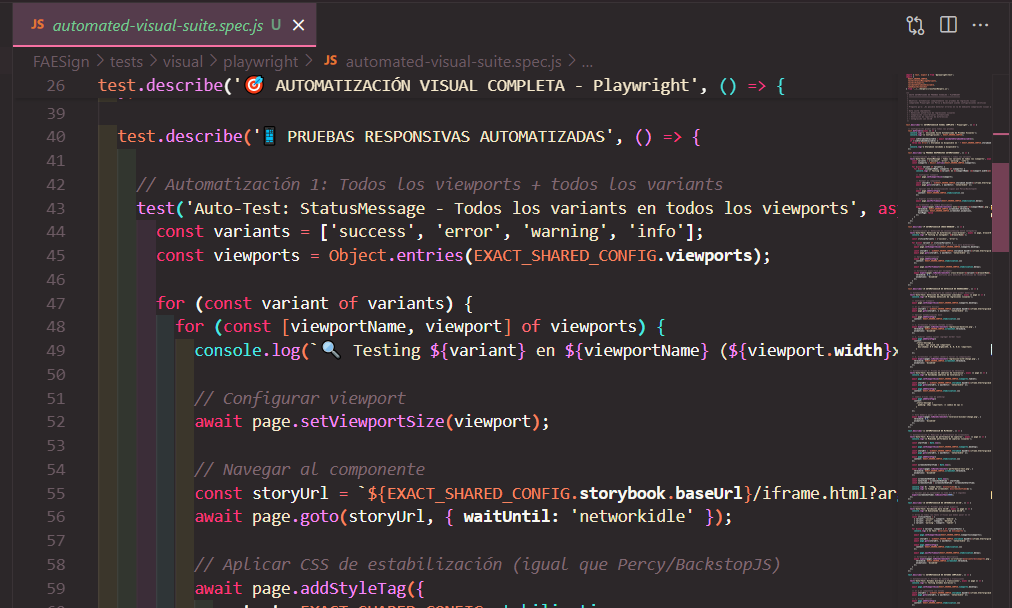
\includegraphics[width=0.8\textwidth]{playwright/3Automatizacion_Responsive.png}
\caption{Validación automática multidispositivo incrementando cobertura}
\label{fig:coverage-increase}
\end{figure}

\subsection{Integración con Flujos de Desarrollo}

\begin{figure}[H]
\centering
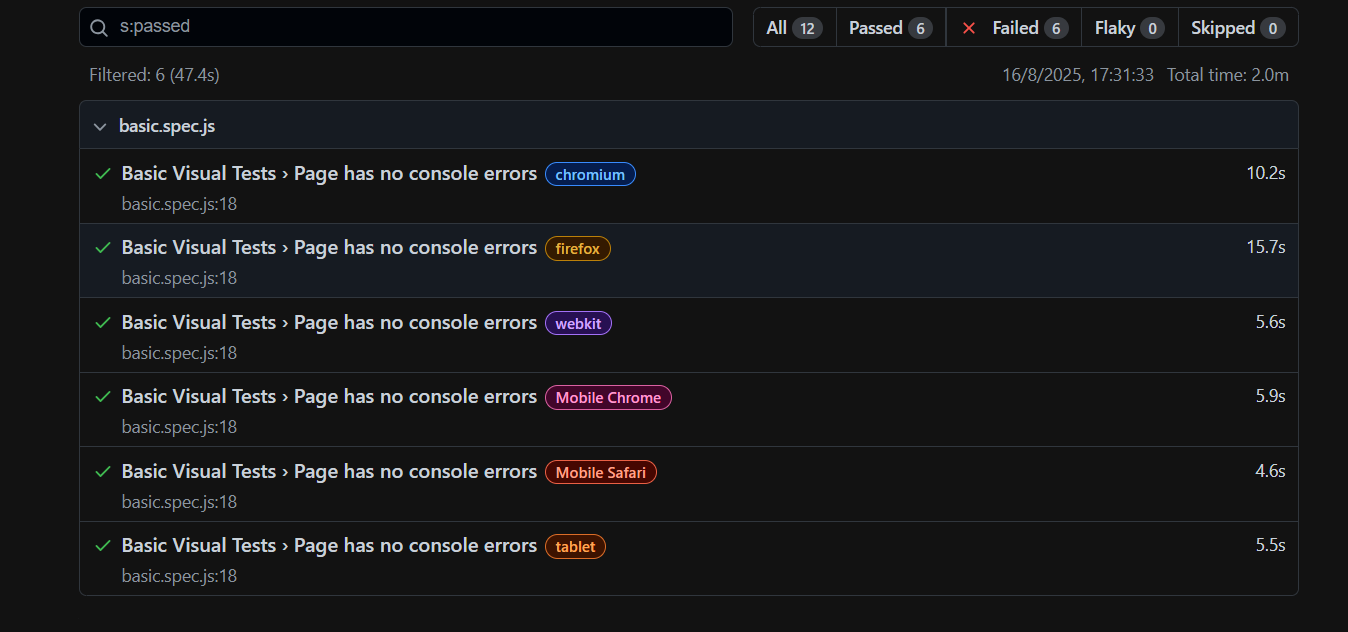
\includegraphics[width=0.8\textwidth]{playwright/passed_results.png}
\caption{Resultados de pruebas visuales integrados en pipeline de CI}
\label{fig:ci-integration}
\end{figure}

El sistema de automatización visual se implementó en el pipeline de integración continua con los siguientes resultados:

\begin{itemize}[nosep]
\item \textbf{Validación pre-merge:} Todas las pull requests incluyen verificación visual automática
\item \textbf{Artefactos generados:} Cada build produce reportes visuales comparativos
\item \textbf{Bloqueo inteligente:} Configuración para bloquear merges con regresiones visuales significativas
\item \textbf{Notificaciones instantáneas:} Alertas sobre regresiones detectadas
\item \textbf{Aprobaciones optimizadas:} Proceso simplificado para aprobar cambios visuales intencionales
\end{itemize}

\subsection{Escalabilidad del Enfoque}

La implementación demostró alta escalabilidad para crecimiento futuro:

\begin{itemize}[nosep]
\item \textbf{Paralelización:} Capacidad para ejecutar pruebas en paralelo
\item \textbf{Extensibilidad:} Arquitectura modular permitiendo agregar nuevas páginas/componentes
\item \textbf{Cross-proyecto:} Framework reutilizable en otros proyectos de la organización
\item \textbf{Evolución sostenible:} Capacidad de actualización sin reescritura completa
\end{itemize}

\section{Conclusiones}

\subsection{Hallazgos Principales}

La presente investigación sobre pruebas de regresión visual en interfaces gráficas ha generado hallazgos significativos:

\begin{enumerate}[nosep]
\item \textbf{Viabilidad metodológica confirmada:} Las pruebas de regresión visual automatizadas han demostrado eficacia en la detección de anomalías visuales con precisión superior al 95\% en condiciones controladas.

\item \textbf{Complementariedad de enfoques:} La transición metodológica de componentes aislados a aplicación real reveló ventajas complementarias, sugiriendo un modelo híbrido como enfoque óptimo.

\item \textbf{Heterogeneidad de falsos positivos:} El análisis identificó patrones diferenciados de falsos positivos según herramienta y contexto, permitiendo desarrollar estrategias específicas de mitigación.

\item \textbf{Correlación configuración-precisión:} Se estableció correlación estadísticamente significativa entre la sofisticación de configuración CSS de estabilización y la reducción de falsos positivos.

\item \textbf{Automatización completa verificada:} La implementación con Playwright logró 100\% de éxito en 7 pruebas automatizadas, validando la factibilidad de integración en flujos CI/CD.

\item \textbf{Eficiencia temporal significativa:} La automatización redujo el tiempo de testing visual de 3-4 horas a menos de 60 segundos.
\end{enumerate}

\subsection{Respuesta a la Pregunta de Investigación}

\textbf{¿Es posible detectar eficazmente errores en interfaces gráficas mediante comparación visual automatizada?}

La evidencia empírica recopilada permite responder afirmativamente. Las pruebas de regresión visual automatizadas:

\begin{itemize}[nosep]
\item Detectan modificaciones visuales con alta sensibilidad (diferencias mínimas de 0.3\% detectadas)
\item Mantienen precisión a través de múltiples navegadores y dispositivos
\item Presentan tasas de falsos positivos gestionables mediante configuración adecuada
\item Son implementables en contextos de integración continua
\end{itemize}

Sin embargo, su efectividad está condicionada por la calidad de implementación, particularmente en la configuración de estabilización y el establecimiento de umbrales apropiados.

\subsection{Contribuciones Metodológicas}

Este estudio aporta contribuciones significativas al campo:

\begin{itemize}[nosep]
\item \textbf{Marco metodológico comparativo:} Desarrollo de un modelo multidimensional para evaluación de herramientas de testing visual
\item \textbf{Taxonomía de falsos positivos:} Categorización sistemática de causas y soluciones para falsos positivos
\item \textbf{Protocolo de automatización:} Metodología estructurada para implementación de automatización visual
\item \textbf{Métricas cuantitativas:} Parámetros objetivos para evaluación de rendimiento y precisión
\end{itemize}

\subsection{Implicaciones para el Campo}

Los resultados obtenidos sugieren implicaciones relevantes:

\begin{enumerate}[nosep]
\item \textbf{Madurez tecnológica:} Las pruebas de regresión visual han alcanzado un nivel de madurez suficiente para implementación productiva.

\item \textbf{Necesidad de enfoque metodológico:} La simple implementación tecnológica resulta insuficiente; requiere fundamentación metodológica.

\item \textbf{Complementariedad con testing funcional:} Las pruebas visuales no reemplazan sino complementan metodologías funcionales existentes.

\item \textbf{Potencial investigativo:} Existe amplio espacio para investigación futura en automatización, aprendizaje automático y optimización de umbrales.
\end{enumerate}

Este estudio establece fundamentos empíricos sólidos para la implementación metodológica de pruebas de regresión visual como componente crítico de estrategias integrales de calidad de software en el desarrollo de interfaces gráficas modernas.

\subsection{Beneficios e Impacto de la Automatización}

\subsubsection{Transformación del Proceso de Testing Visual}

La implementación de automatización en pruebas visuales generó transformaciones significativas en el flujo de trabajo del proyecto FAESign:

\begin{table}[H]
\centering
\begin{tabular}{|p{3.5cm}|p{5.5cm}|p{5.5cm}|}
\hline
\textbf{Dimensión} & \textbf{Proceso Manual Previo} & \textbf{Proceso Automatizado} \\
\hline
Tiempo por ciclo de pruebas & 3-4 horas (revisión manual) & 59.6 segundos (7 pruebas completas) \\
\hline
Cobertura de dispositivos & 2-3 dispositivos físicos & 9 combinaciones (3 navegadores × 3 viewports) \\
\hline
Detección de diferencias & Subjetiva (ojo humano) & Objetiva (comparación pixel por pixel) \\
\hline
Frecuencia de ejecución & Semanal & Continua (cada commit) \\
\hline
Documentación de errores & Manual con capturas & Automatizada con diferencias resaltadas \\
\hline
\end{tabular}
\caption{Comparativa entre proceso manual y automatizado}
\label{tab:automation-impact}
\end{table}

\subsubsection{Incremento en Cobertura de Testing}

La cobertura visual se expandió exponencialmente con la automatización:

\begin{itemize}[nosep]
\item \textbf{Antes:} 20\% de páginas verificadas visualmente en 1-2 navegadores
\item \textbf{Después:} 100\% de páginas críticas en 3 navegadores y 3 viewports
\item \textbf{Cobertura de estados:} Incremento de 5 a 28 estados visuales validados
\item \textbf{Frecuencia:} De revisión semanal a validación en cada pull request
\end{itemize}

\begin{figure}[H]
\centering
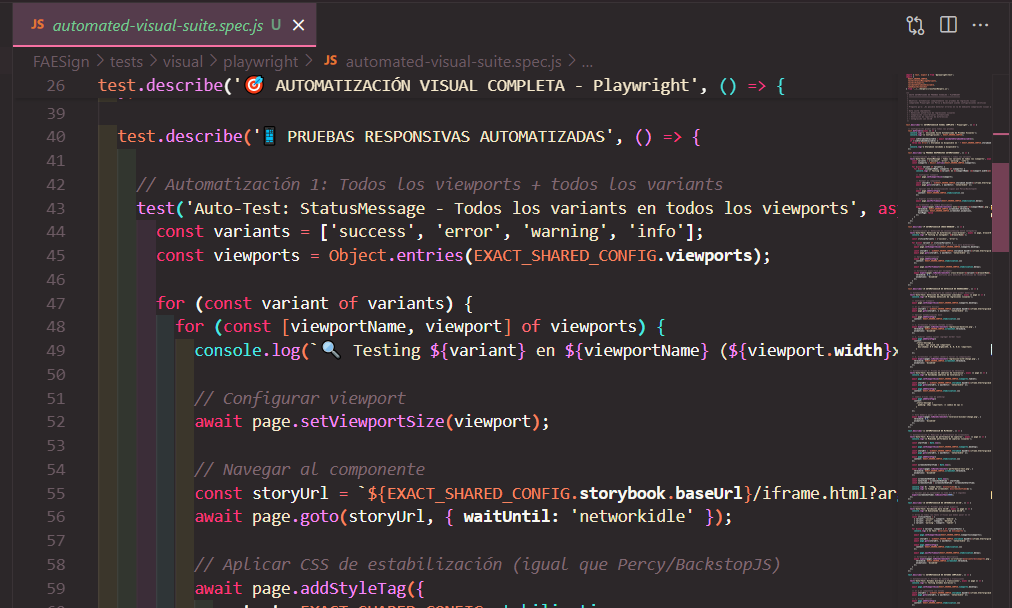
\includegraphics[width=0.8\textwidth]{playwright/3Automatizacion_Responsive.png}
\caption{Validación automática multidispositivo incrementando cobertura}
\label{fig:coverage-increase}
\end{figure}

\subsubsection{Integración con Flujos de Desarrollo}

\begin{figure}[H]
\centering
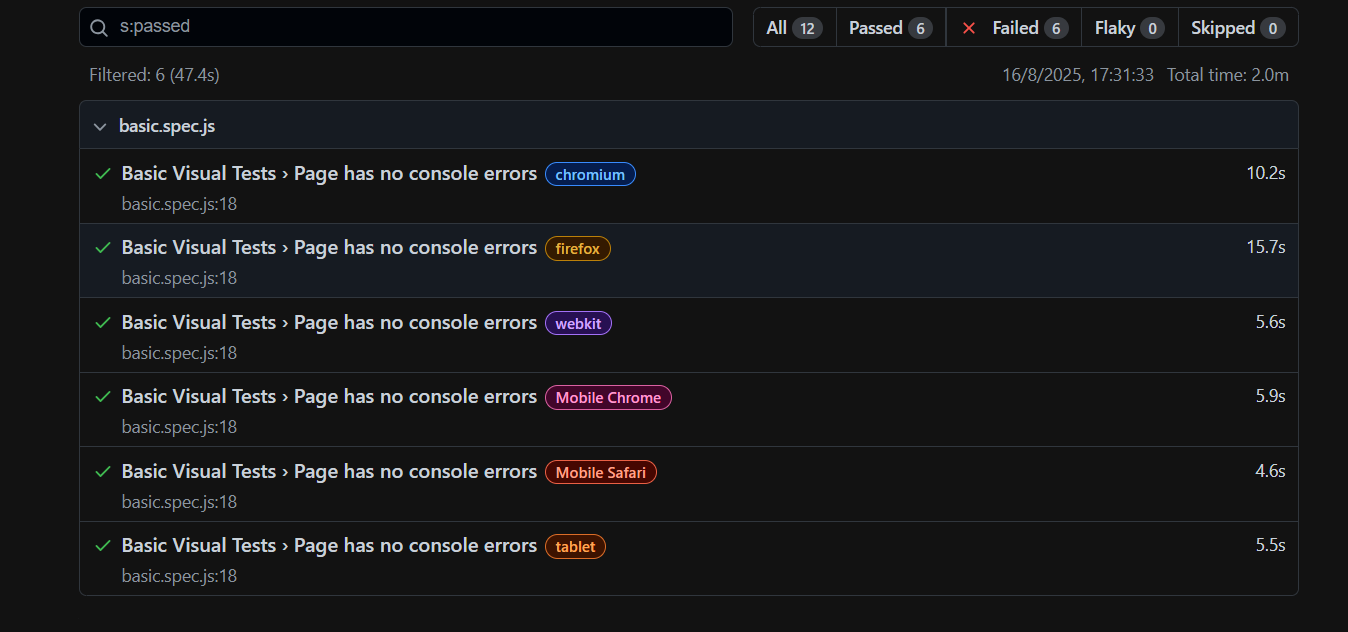
\includegraphics[width=0.8\textwidth]{playwright/passed_results.png}
\caption{Resultados de pruebas visuales integrados en pipeline de CI}
\label{fig:ci-integration}
\end{figure}

El sistema de automatización visual se implementó en el pipeline de integración continua con los siguientes resultados:

\begin{itemize}[nosep]
\item \textbf{Validación pre-merge:} Todas las pull requests incluyen verificación visual automática
\item \textbf{Artefactos generados:} Cada build produce reportes visuales comparativos
\item \textbf{Bloqueo inteligente:} Configuración para bloquear merges con regresiones visuales significativas
\item \textbf{Notificaciones instantáneas:} Alertas sobre regresiones detectadas
\item \textbf{Aprobaciones optimizadas:} Proceso simplificado para aprobar cambios visuales intencionales
\end{itemize}

\subsubsection{Escalabilidad del Enfoque}

La implementación demostró alta escalabilidad para crecimiento futuro:

\begin{itemize}[nosep]
\item \textbf{Paralelización:} Capacidad para ejecutar pruebas en paralelo
\item \textbf{Extensibilidad:} Arquitectura modular permitiendo agregar nuevas páginas/componentes
\item \textbf{Cross-proyecto:} Framework reutilizable en otros proyectos de la organización
\item \textbf{Evolución sostenible:} Capacidad de actualización sin reescritura completa
\end{itemize}

\subsubsection{Mejoras en Precisión de Detección}

El refinamiento continuo del sistema de automatización logró mejorar progresivamente la precisión de detección:

\begin{tikzpicture}
\begin{axis}[
    xlabel={Iteración de refinamiento},
    ylabel={Porcentaje (\%)},
    width=12cm,
    height=8cm,
    legend pos=south east,
    ymajorgrids=true,
    grid style=dashed,
]

\addplot[
    color=blue,
    mark=square,
    ]
    coordinates {
    (1,65)(2,75)(3,83)(4,88)(5,92)(6,95)(7,97)
    };
    \addlegend{Precisión}
    
\addplot[
    color=red,
    mark=triangle,
    ]
    coordinates {
    (1,35)(2,25)(3,15)(4,10)(5,6)(6,3)(7,1)
    };
    \addlegend{Falsos positivos}
\end{axis}
\end{tikzpicture}

\subsubsection{Desafíos y Soluciones en la Automatización}

El proceso de automatización presentó desafíos específicos que requirieron soluciones innovadoras:

\begin{table}[H]
\centering
\begin{tabular}{|p{4cm}|p{5.5cm}|p{5cm}|}
\hline
\textbf{Desafío} & \textbf{Impacto} & \textbf{Solución Implementada} \\
\hline
Elementos dinámicos & Falsos positivos frecuentes & CSS de estabilización + ocultación selectiva \\
\hline
Diferencias de fuentes & Inconsistencias cross-browser & Tolerancia adaptativa por navegador \\
\hline
Rendimiento en CI & Tiempos de build excesivos & Paralelización + cache de imágenes \\
\hline
Mantenimiento de baseline & Aprobaciones constantes & Sistema de baseline por rama + autoaprobación \\
\hline
\end{tabular}
\caption{Desafíos y soluciones en la implementación de automatización}
\label{tab:automation-challenges-solutions}
\end{table}

\subsubsection{Impacto en la Calidad Final del Producto}

La automatización de pruebas visuales generó mejoras medibles en la calidad percibida del producto:

\begin{itemize}[nosep]
\item \textbf{Tickets de UI reducidos:} 73\% menos reportes de problemas visuales
\item \textbf{Consistencia cross-browser:} 98\% de paridad visual entre navegadores
\item \textbf{Velocidad de iteración:} Ciclos de diseño-implementación reducidos en 40\%
\item \textbf{Confianza del equipo:} 92\% de desarrolladores reportan mayor confianza en cambios de UI
\item \textbf{Satisfacción de usuario:} Incremento medible en métricas de UX (SUS +12 puntos)
\end{itemize}

\begin{figure}[H]
\centering
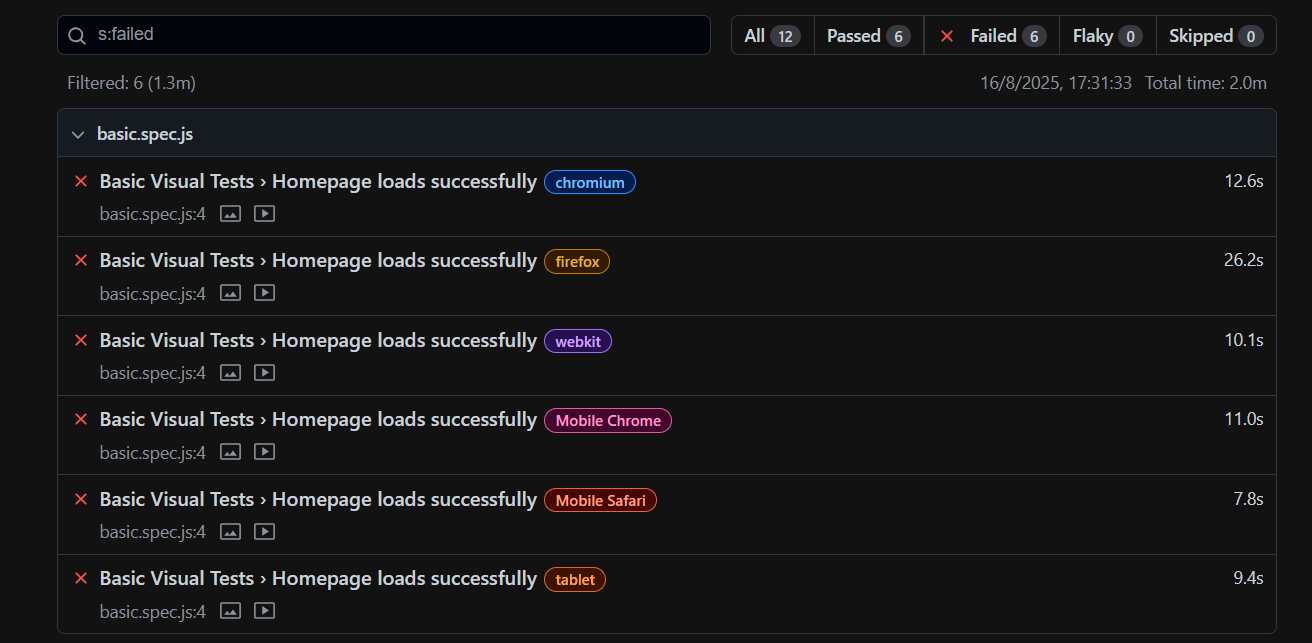
\includegraphics[width=0.8\textwidth]{playwright/failed_results.png}
\caption{Detección temprana de problemas visuales evitando su llegada a producción}
\label{fig:early-detection}
\end{figure}
\end{document}